%% fcup-thesis.tex -- document template for PhD theses at FCUP
%%
%% Copyright (c) 2015 João Faria <joao.faria@astro.up.pt>
%%
%% This work may be distributed and/or modified under the conditions of
%% the LaTeX Project Public License, either version 1.3c of this license
%% or (at your option) any later version.
%% The latest version of this license is in
%%     http://www.latex-project.org/lppl.txt
%% and version 1.3c or later is part of all distributions of LaTeX
%% version 2005/12/01 or later.
%%
%% This work has the LPPL maintenance status "maintained".
%%
%% The Current Maintainer of this work is
%% João Faria <joao.faria@astro.up.pt>.
%%
%% This work consists of the files listed in the accompanying README.

%% SUMMARY OF FEATURES:
%%
%% All environments, commands, and options provided by the `ut-thesis'
%% class will be described below, at the point where they should appear
%% in the document.  See the file `ut-thesis.cls' for more details.
%%
%% To explicitly set the pagestyle of any blank page inserted with
%% \cleardoublepage, use one of \clearemptydoublepage,
%% \clearplaindoublepage, \clearthesisdoublepage, or
%% \clearstandarddoublepage (to use the style currently in effect).
%%
%% For single-spaced quotes or quotations, use the `longquote' and
%% `longquotation' environments.


%%%%%%%%%%%%         PREAMBLE         %%%%%%%%%%%%

%%  - Default settings format a final copy (single-sided, normal
%%    margins, one-and-a-half-spaced with single-spaced notes).
%%  - For a rough copy (double-sided, normal margins, double-spaced,
%%    with the word "DRAFT" printed at each corner of every page), use
%%    the `draft' option.
%%  - The default global line spacing can be changed with one of the
%%    options `singlespaced', `onehalfspaced', or `doublespaced'.
%%  - Footnotes and marginal notes are all single-spaced by default, but
%%    can be made to have the same spacing as the rest of the document
%%    by using the option `standardspacednotes'.
%%  - The size of the margins can be changed with one of the options:
%%     . `narrowmargins' (1 1/4" left, 3/4" others),
%%     . `normalmargins' (1 1/4" left, 1" others),
%%     . `widemargins' (1 1/4" all),
%%     . `extrawidemargins' (1 1/2" all).
%%  - The pagestyle of "cleared" pages (empty pages inserted in
%%    two-sided documents to put the next page on the right-hand side)
%%    can be set with one of the options `cleardoublepagestyleempty',
%%    `cleardoublepagestyleplain', or `cleardoublepagestylestandard'.
%%  - Any other standard option for the `report' document arclass can be
%%    used to override the default or draft settings (such as `10pt',
%%    `11pt', `12pt'), and standard LaTeX packages can be used to
%%    further customize the layout and/or formatting of the document.

%% *** Add any desired options. ***
%PDF
%\documentclass[a4paper,narrowmargins,11pt,oneside,draft,onehalfspaced,singlespacednotes]{fcup-thesis}
%\documentclass[a4paper,narrowmargins,11pt,oneside,onehalfspaced,singlespacednotes]{fcup-thesis}
%Print
%\documentclass[draft,a4paper,narrowmargins,11pt,twoside,openright,onehalfspaced,singlespacednotes]{fcup-thesis}
\documentclass[a4paper,narrowmargins,11pt,twoside,openright,onehalfspaced,singlespacednotes]{fcup-thesis}

%% *** Add \usepackage declarations here. ***
%% The standard packages `geometry' and `setspace' are already loaded by
%% `ut-thesis' -- see their documentation for details of the features
%% they provide.  In particular, you may use the \geometry command here
%% to adjust the margins if none of the ut-thesis options are suitable
%% (see the `geometry' package for details).  You may also use the
%% \setstretch command to set the line spacing to a value other than
%% single, one-and-a-half, or double spaced (see the `setspace' package
%% for details).
% Overfull statements
\pretolerance=150
\setlength{\emergencystretch}{3em}
% Overfull end
\usepackage[english]{babel}
\usepackage{helvet} %To replace arial fonts
\usepackage{lipsum}
\usepackage[utf8]{inputenc}


%%% Additional useful packages
%%% ----------------------------------------------------------------
\usepackage{array}
\usepackage{amsmath}  
\usepackage{amssymb}
\usepackage{amsfonts}
\DeclareFontFamily{OT1}{pzc}{}
\DeclareFontShape{OT1}{pzc}{m}{it}{<-> s * [0.900] pzcmi7t}{}
\DeclareMathAlphabet{\mathpzc}{OT1}{pzc}{m}{it}
%Titles need to be 14 pt => Large in \normaltext 11pt
\usepackage{titlesec}
\titleformat*{\section}{\Large\bfseries}
\titleformat*{\subsection}{\Large\bfseries}
\titleformat*{\subsubsection}{\Large\bfseries}
%Titles need to be 14 pt => Large in \normaltext 11pt
\usepackage{amsthm}      
\usepackage[ruled,algochapter]{algorithm2e}
\usepackage{algorithmic}
\usepackage{bm}
\usepackage[mathscr]{euscript}
\usepackage{graphicx}       
\usepackage{psfrag}         
\usepackage{fancyvrb}    
\usepackage{float}
\usepackage{ltablex}
\usepackage[square,sort,comma,numbers]{natbib}        
\usepackage{bbding}         
\usepackage{dcolumn}        
\usepackage{booktabs} 
\usepackage{multirow}
\usepackage{paralist}     
\usepackage{ifdraft}  
\usepackage{indentfirst}    
\usepackage[nottoc,notlof,notlot]{tocbibind}
\usepackage{url}
\usepackage{tabularx}
%use font size for captions like 8pt -> normalisize 11pt, scriptsize->8pt
\usepackage[font={scriptsize}]{caption}
\usepackage[font={scriptsize}]{subcaption}
\captionsetup{font=scriptsize}

\usepackage[unicode]{hyperref}
\usepackage{xcolor}


\hypersetup{pdftitle=Obstacle avoidance framework based on reach sets, 
            pdfauthor=Alojz Gomola,
            colorlinks=false,
            urlcolor=blue,
            pdfstartview=FitH,
            pdfpagemode=UseOutlines,
            pdfnewwindow,
            breaklinks
          }
\usepackage{array}
\newcolumntype{L}[1]{>{\raggedright\let\newline\\\arraybackslash\hspace{0pt}}m{#1}}
\newcolumntype{C}[1]{>{\centering\let\newline\\\arraybackslash\hspace{0pt}}m{#1}}
\newcolumntype{R}[1]{>{\raggedleft\let\newline\\\arraybackslash\hspace{0pt}}m{#1}}         
\newcolumntype{B}{X}
\newcolumntype{S}[1]{>{\hsize=#1\textwidth}X}

\newcommand{\FIGDIR}{./Pics}    %%% directory containing figures
\newcommand{\twolinecellr}[2][r]{%
  \begin{tabular}[#1]{@{}r@{}}#2\end{tabular}}
\newcommand{\secState}[1]{
	\ifdraft{(#1) }{}
}
\theoremstyle{plain}
\newtheorem{theorem}{Theorem}
\newtheorem{lemma}[theorem]{Lemma}
\newtheorem{proposition}[theorem]{Proposition}

\theoremstyle{plain}
\newtheorem{definition}{Definition}
\newtheorem{problem}{Problem}
\newtheorem{example}{Example}
\newtheorem{assumption}{Assumption}

\theoremstyle{remark}
\newtheorem*{corollary}{Corollary}
\newtheorem*{note}{Note}




\newenvironment{dokaz}{
  \par\medskip\noindent
  \textit{Proof}.
}{
\newline
\rightline{\SquareCastShadowBottomRight}
}

\newenvironment{constraints}[1]{
  \par\medskip\noindent
  \textit{Constraints #1} \\
}{
\newline
\rightline{\SquareCastShadowBottomRight}
}


%\bibliographystyle{plainnat}     %% Author (year) style
\bibliographystyle{unsrt}        %% [number] style
\setcitestyle{square}

% Section  3.7 Challenge list
\newif\ifproblemchallenge   %# Build block for problem challenges
\problemchallengetrue       %# Show comments

\newcommand{\R}{\mathbb{R}}
\newcommand{\N}{\mathbb{N}}

\DeclareMathOperator{\pr}{\textsf{P}}
\DeclareMathOperator{\E}{\textsf{E}\,}
\DeclareMathOperator{\var}{\textrm{var}}
\DeclareMathOperator{\sd}{\textrm{sd}}


\newcommand{\T}[1]{#1^\top}        

\newcommand{\goto}{\rightarrow}
\newcommand{\gotop}{\stackrel{P}{\longrightarrow}}
\newcommand{\maon}[1]{o(n^{#1})}
\newcommand{\abs}[1]{\left|{#1}\right|}
\newcommand{\dint}{\int_0^\tau\!\!\int_0^\tau}
\newcommand{\isqr}[1]{\frac{1}{\sqrt{#1}}}
\newcommand{\norm}[1]{\left\lVert#1\right\rVert}


\newcommand{\pulrad}[1]{\raisebox{1.5ex}[0pt]{#1}}
\newcommand{\mc}[1]{\multicolumn{1}{c}{#1}}
\newcommand{\TBD}[1]{\color{red}\emph{--TBD:}#1\color{black}}

%%%%%%%%%%%%%%%%%%%%%%%%%%%%%%%%%%%%%%%%%%%%%%%%%%%%%%%%%%%%%%%%%%%%%%%%
%%                                                                    %%
%%                   ***   I M P O R T A N T   ***                    %%
%%                                                                    %%
%%  Fill in the following fields with the required information:       %%
%%   - \degree{...}       name of the degree obtained                 %%
%%   - \department{...}   name of the graduate department             %%
%%   - \gradyear{...}     year of graduation                          %%
%%   - \author{...}       name of the author                          %%
%%   - \title{...}        title of the thesis                         %%
%%%%%%%%%%%%%%%%%%%%%%%%%%%%%%%%%%%%%%%%%%%%%%%%%%%%%%%%%%%%%%%%%%%%%%%%

%% *** Change this example to appropriate values. ***
\degree{Doctor of Philosophy}
\department{Departamento de Matem\'{a}tica}
\gradyear{2019}
\author{Alojz Gomola}
\title{Obstacle Avoidance Framework based on Reach Sets}

%% *** NOTE ***
%% Put here all other formatting commands that belong in the preamble.
%% In particular, you should put all of your \newcommand's,
%% \newenvironment's, \newtheorem's, etc. (in other words, all the
%% global definitions that you will need throughout your thesis) in a
%% separate file and use "\input{filename}" to input it here.


%% *** Adjust the following settings as desired. ***

%% List only down to subsections in the table of contents;
%% 0=chapter, 1=section, 2=subsection, 3=subsubsection, etc.
\setcounter{tocdepth}{3}

%% Make each page fill up the entire page.
\flushbottom


%%%%%%%%%%%%      MAIN  DOCUMENT      %%%%%%%%%%%%

\begin{document}


%%%%%%%%%%%%%%%%%%%%%%%%%%%%%%%%%%%%%%%%%%%%%%%%%%%%%%%%%%%%%%%%%%%%%%%%
%%  Put your Chapters here; the easiest way to do this is to keep     %%
%%  each chapter in a separate file and `\include' all the files.     %%
%%  Each chapter file should start with "\chapter{ChapterName}".      %%
%%  Note that using `\include' instead of `\input' will make each     %%
%%  chapter start on a new page, and allow you to format only parts   %%
%%  of your thesis at a time by using `\includeonly'.                 %%
%%%%%%%%%%%%%%%%%%%%%%%%%%%%%%%%%%%%%%%%%%%%%%%%%%%%%%%%%%%%%%%%%%%%%%%%

%% *** Include chapter files here. ***

\setcounter{chapter}{6}
\setcounter{section}{6}
%06-Approach
   
   
    
    %06-08 UTM implementation
		\cleardoublepage
\section{UTM Prototype Implementation}\label{sec:UASTrafficManagement}

\noindent The \emph{Traffic Management} for UAS is based on existing Air Traffic Management System for manned aviation \cite{icao4444}. The controlled airspace segments are \emph{static} and have one \emph{authority for one zone} principle. The dynamic zones have been proposed in \cite{gerdes2016dynamic}. However, it will be omitted for \emph{simplification purpose}. The necessity for \emph{UAS integration} into \emph{National Airspace} has been outlined in \cite{spriesterbach2013unmanned}.

The latest \emph{Airbus blueprint} \cite{airbusUTM2018blueprint} outlines some functionality. The main purpose of this section is to show \emph{Reach Set based Approach} capability to follow \emph{Usual Air Traffic Management} commands.

The \emph{section} is organized to introduce:
\begin{enumerate}
    \item \emph{UTM Architecture} (sec. \ref{sec:utmArchitecture}) - centralized ATM-like authority over airspace cluster.
    
    \item \emph{Handling Standard Collision Situations} - head-on approach (sec. \ref{sec:handlingHeadOnApproach}), converging situation (sec. \ref{sec:handlingConvergingManuever}), overtake (sec. \ref{sec:handlingOvertakeManuever}).
    
    \item \emph{Position Notification} (sec. \ref{sec:positionNotification}) - position notification design.
    
    \item \emph{Collision Case} (sec. \ref{sec:collisionCase}) - calculation and handling of \emph{collision situations}.
    
\end{enumerate}

\noindent The additional material can be found in:
\begin{enumerate}
	\item \emph{Cooperative Conflict Resolution} (app. \ref{sec:cooperativeConflictResolution}) - the model used for conflict resolution in \emph{controlled airspace}.
    
    \item \emph{Non-Cooperative Conflict Resolution} (app. \ref{sec:nonCooperativeConflictResolution})  - the model used for conflict resolution in \emph{non-controlled} airspace and \emph{emergency avoidance}.
    
    \item \emph{Weather Case} (app. \ref{sec:weatherCase}) - definition and handling of \emph{weather hazards}.
\end{enumerate}
		\subsection{(R) Architecture}
\paragraph{UTM concept} is based on \emph{asynchronous event-based control} \cite{zimmer2011rule}. \emph{Event} in \emph{controlled airspace} is handled in form of \emph{cases} \cite{prevot2016uas}. There are following \emph{event sources}:

\begin{enumerate}
    \item \emph{Weather Information Service} (from \cite{zimmer2014selective}) - used to create \emph{weather case} (tab. \ref{tab:weatherConstraint}).
    
    \item \emph{Position Notification from UAS systems} (tab. \ref{tab:positionNotification}) - used to create \emph{collision cases} (new functionality) (tab. \ref{tab:collisionCase}).
\end{enumerate}


\paragraph{Decision frame} (eq. \ref{eq:decisionFrameDefinition}). The \emph{UTM} is operating in discrete decision frames which are starting on current \emph{decision time} and ending at  next \emph{decision  time}:

\begin{equation}\label{eq:decisionFrameDefinition}
    decision Frame_i = [decision Time_i, decision Time_{i+1}[,\quad i \in {1,\dots,k}, k \in \N^+
\end{equation}

\paragraph{Event based airspace control} is collecting  events in  previous $decisionFrame_{i-1}$ and issuing commands in current $decisionFrame_i$.There are following phases during the \emph{UTM frame} cycle:
\begin{enumerate}
    \item \emph{Planning} - the detection phase, when the hazardous situations are assessed.
    
    \item \emph{Fulfillment} - the monitoring phase, when the state of affairs for directives and mandates is full filled by controlled UAS systems. 
    
    \item \emph{Acknowledgement} - the closing phase, when UTM assess and acknowledges the performance of controlled UAS systems.
\end{enumerate}


\begin{figure}[H]
    \centering
    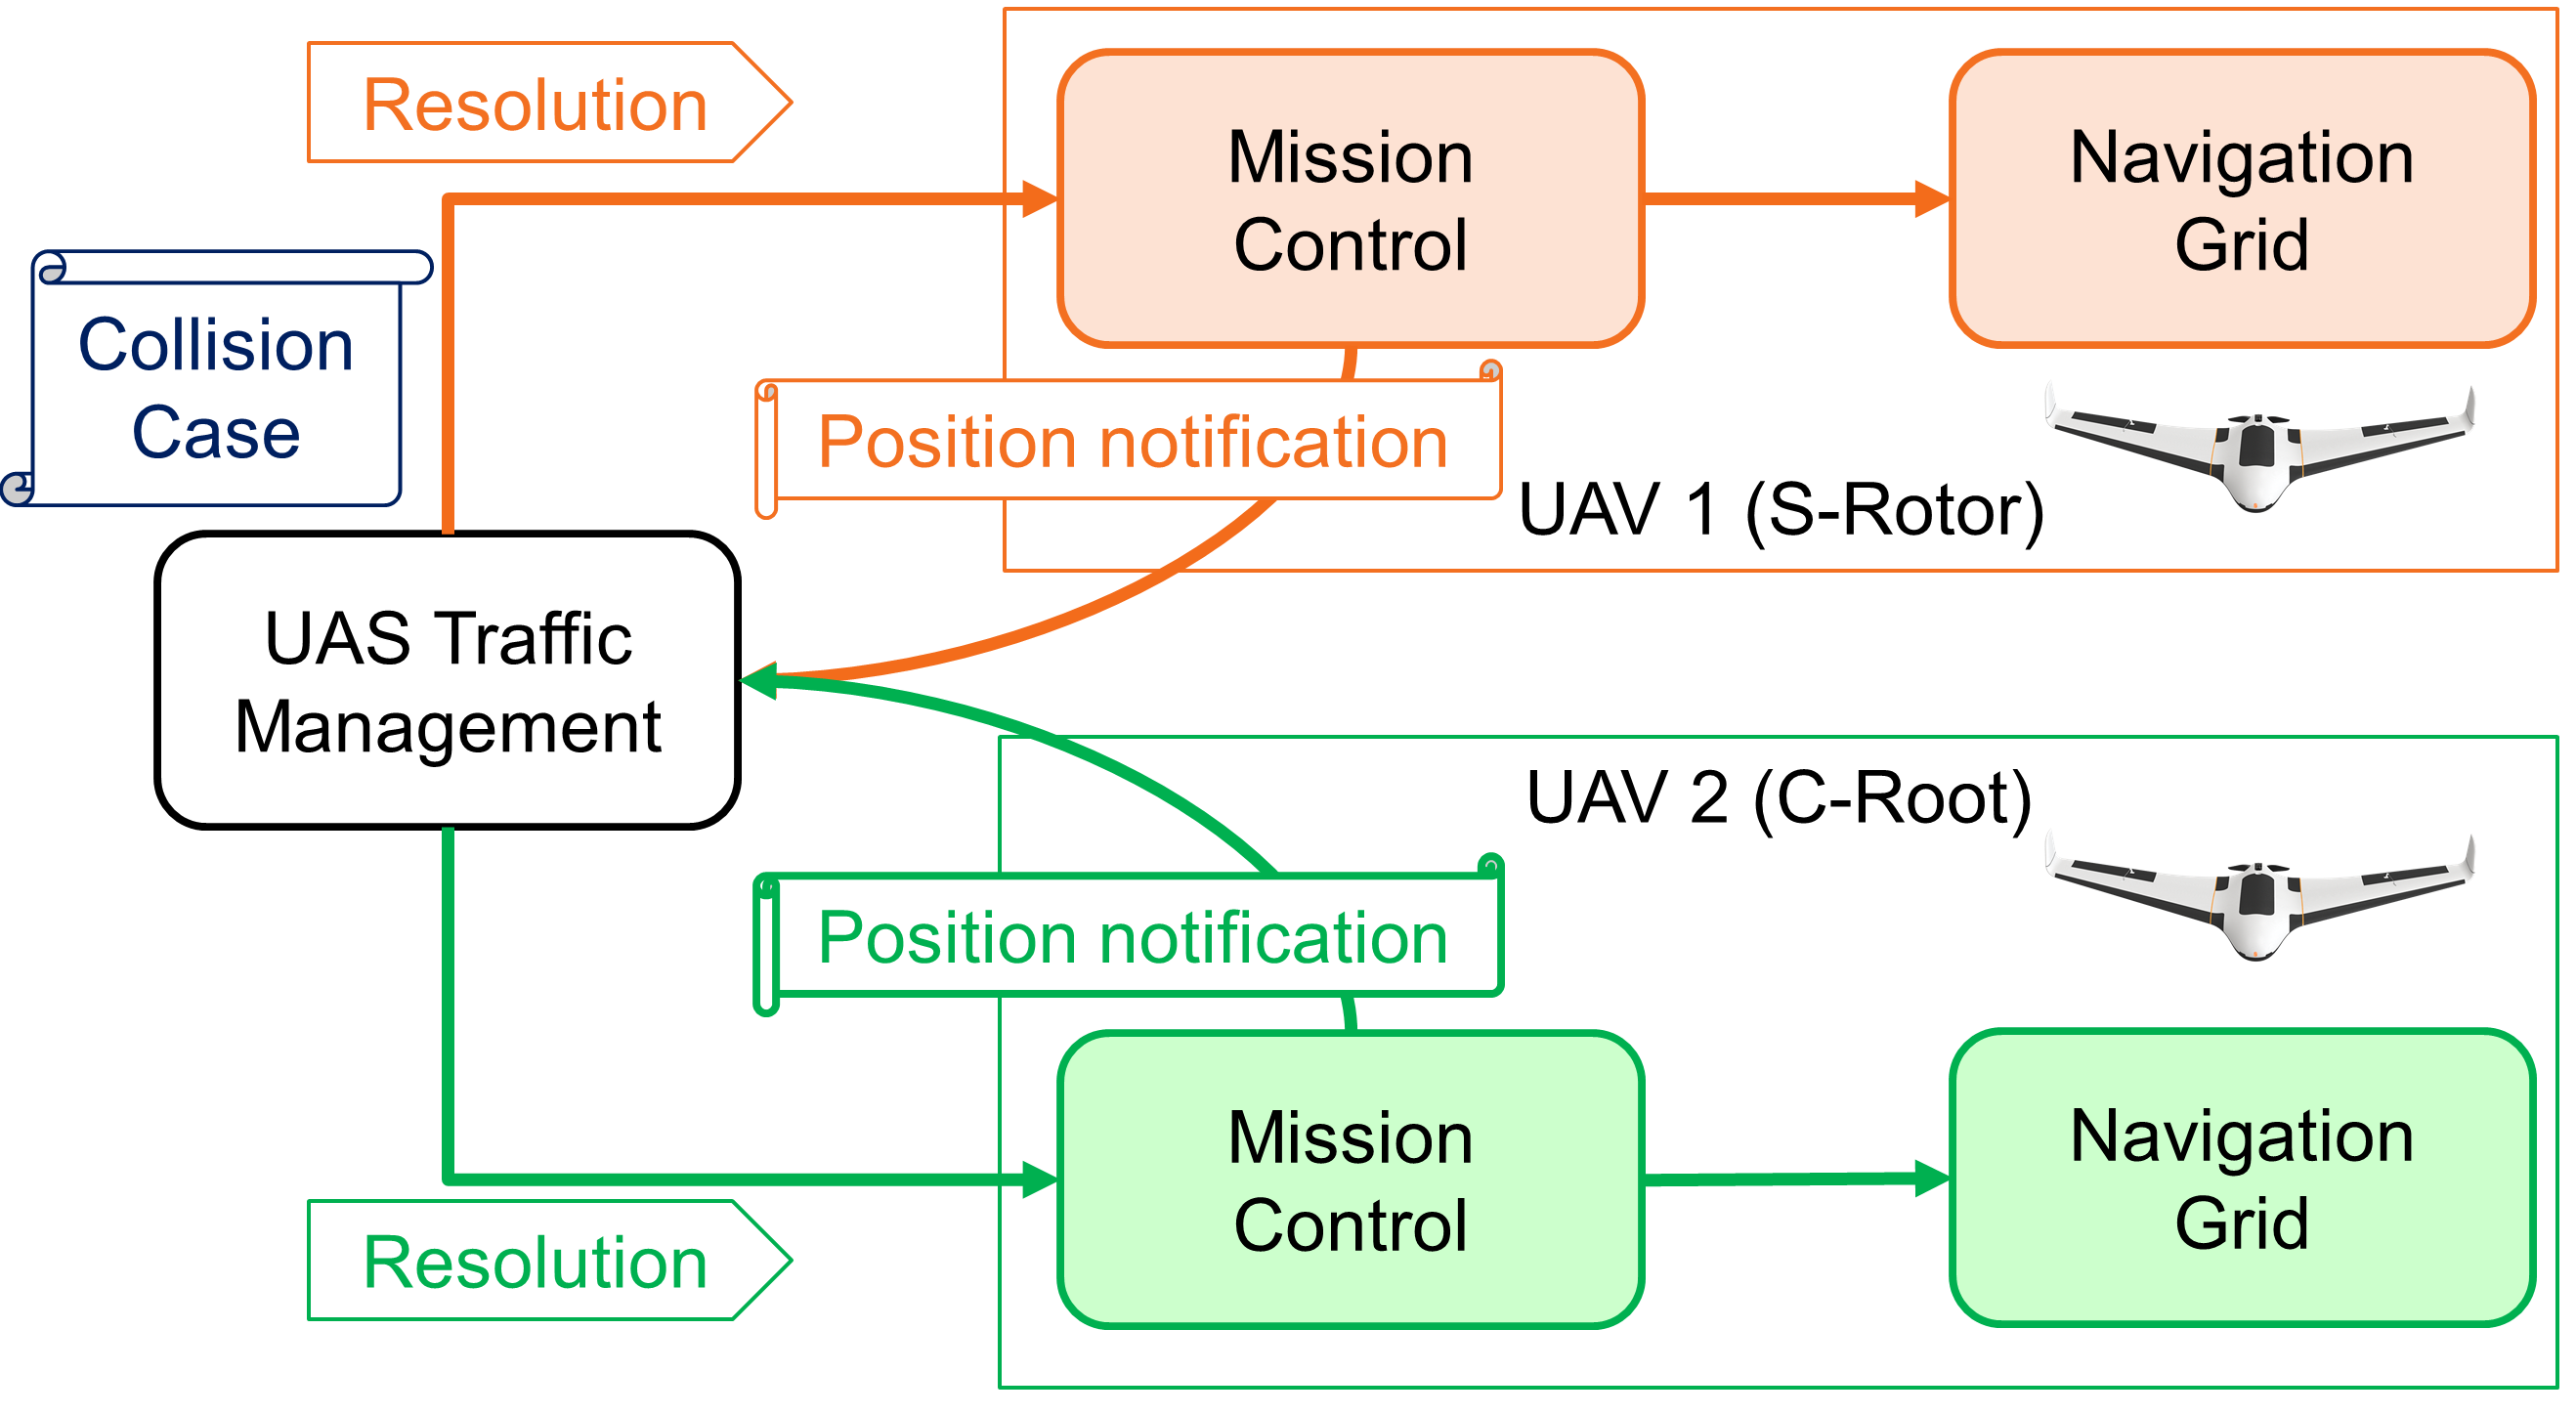
\includegraphics[width=0.7\linewidth]{\FIGDIR/RE002UTMCommunicationDiagram} 
    \caption{UAS Traffic (UTM) Management architecture overview.}
    \label{fig:UTMArchitectureOverview}
\end{figure}

\paragraph{Architecture:} (fig. \ref{fig:UTMArchitectureOverview}).  There are multiple UAS systems equipped with standard \emph{Mission Control} and \emph{Navigation} procedures. 

Depending on the \emph{airspace cluster} decision time frame they are sending \emph{periodical position notifications} (tab. \ref{tab:positionNotification}).

The \emph{UAS Traffic Management} (UTM) collects the event data from \emph{Weather Information Service} and \emph{Position Notifications} calculating respective \emph{cases}. 

If there is an \emph{active collision/weather case} the \emph{UTM} will send \emph{resolutions} to respective airspace attendants. 
		\subsection{Handling Head-on Approach}\label{sec:handlingHeadOnApproach}

\paragraph{Summary:} Two UAS are facing each other head-on. There is a need to define triggers for detection and resolution approach for autonomous UAS.  Rules for VFR/IFR modes in manned aviation are the base for the autonomous collision resolution. The concept of the virtual roundabout is introduced.

\paragraph{Goal:} Identify required parameters sufficient for automatic solution of \emph{Head-on collision} situation.

\paragraph{VFR:} The \emph{Visual Flight Rules} (VFR) are specified in annex 2 \cite{icaoAnnex2}, and there is a \emph{Head-on} approach for two or more air crafts. The definition is rather vague: "The pilot should diverge from original heading to the right to create sufficient, safe space for avoidance." 

\paragraph{IFR:} The \emph{Instrument Flight Rules} in annex 2. \cite{icaoAnnex2} and 11. \cite{icaoAnnex11} are defining the boundaries and events for success full \emph{Head-on resolution} in larger detail. 

The parameter values are useless due to the UAS scaling factor; the following parameters can be used in UTM:

\begin{enumerate}
    \item The \emph{angle of approach $\ge 130^\circ$} - the minimal planar angle between aircraft positions and expected collision point is in the interval $[130^\circ,180^\circ]$.
    
    \item \emph{Minimal detection range} - the minimal detection range of head-on collision is $2\times turning Radius + safety Margin$.
    
    \item \emph{Safety margin} - during avoidance all aircraft keeps mutual distance at least the value of safety margin.
\end{enumerate}

\begin{figure}[H]
	\centering
    \begin{subfigure}{0.45\textwidth}
    	\centering
        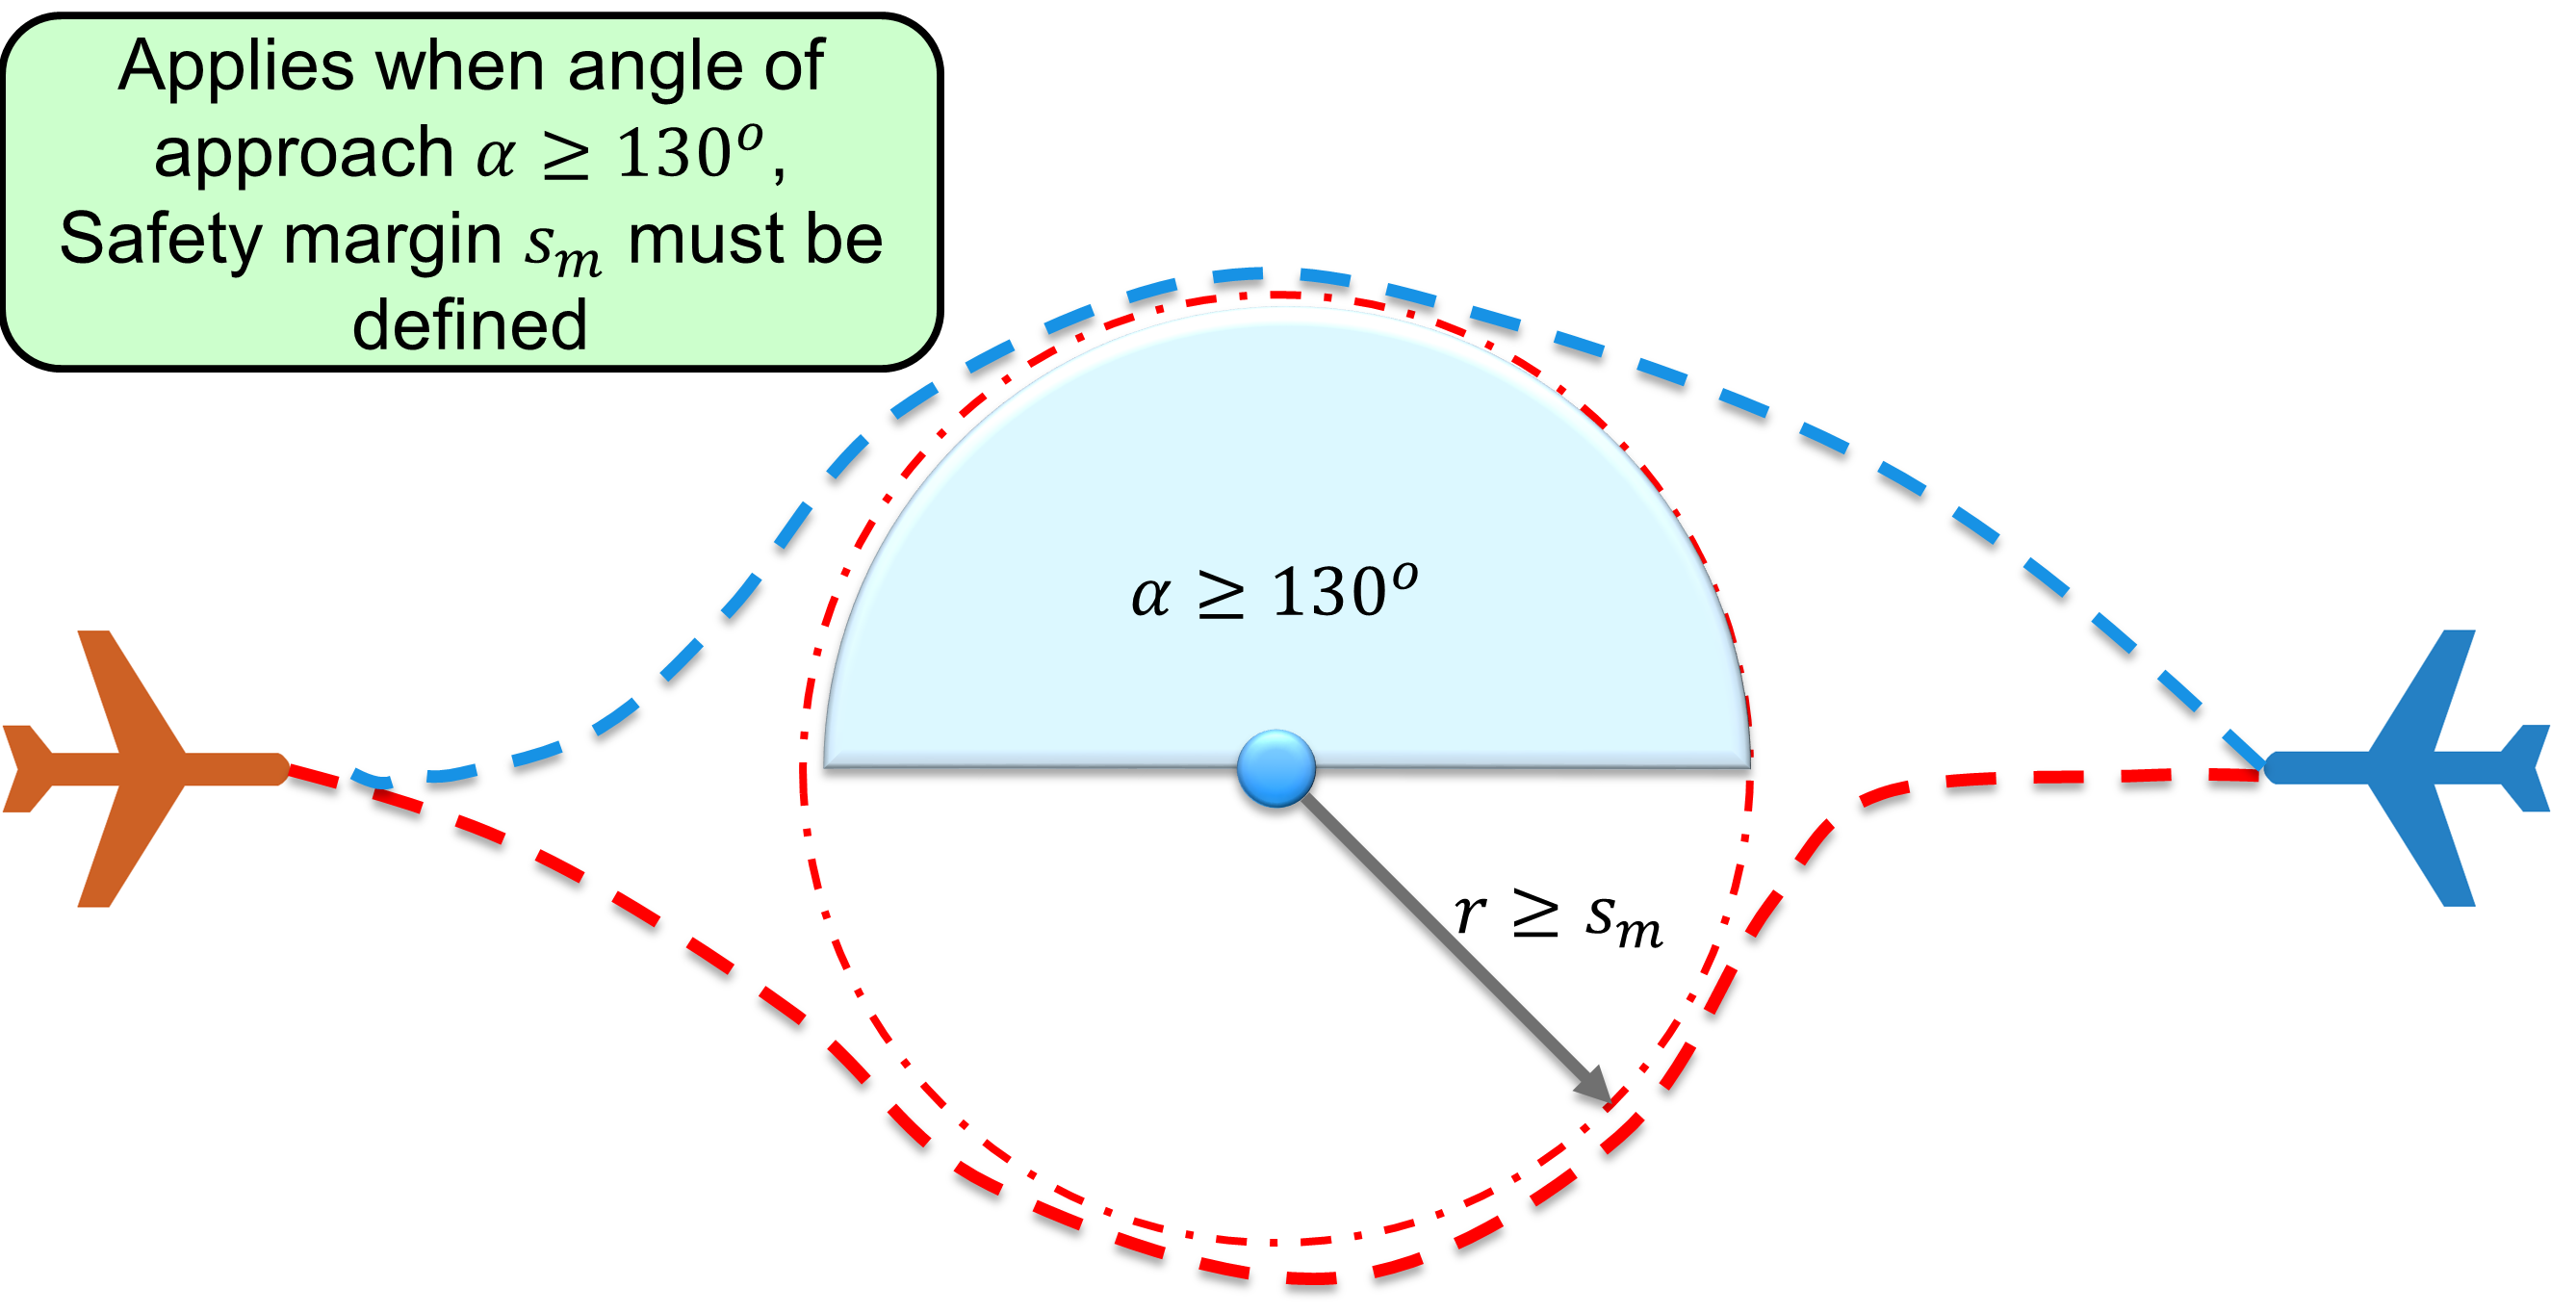
\includegraphics[width=0.9\linewidth,height=95pt,keepaspectratio]{\FIGDIR/RE008HeadOnApproach01} 
        \caption{Detection.}
        \label{fig:HeadOnApproachTheoreticalDetection}
    \end{subfigure}
    \begin{subfigure}{0.45\textwidth}
    	\centering
        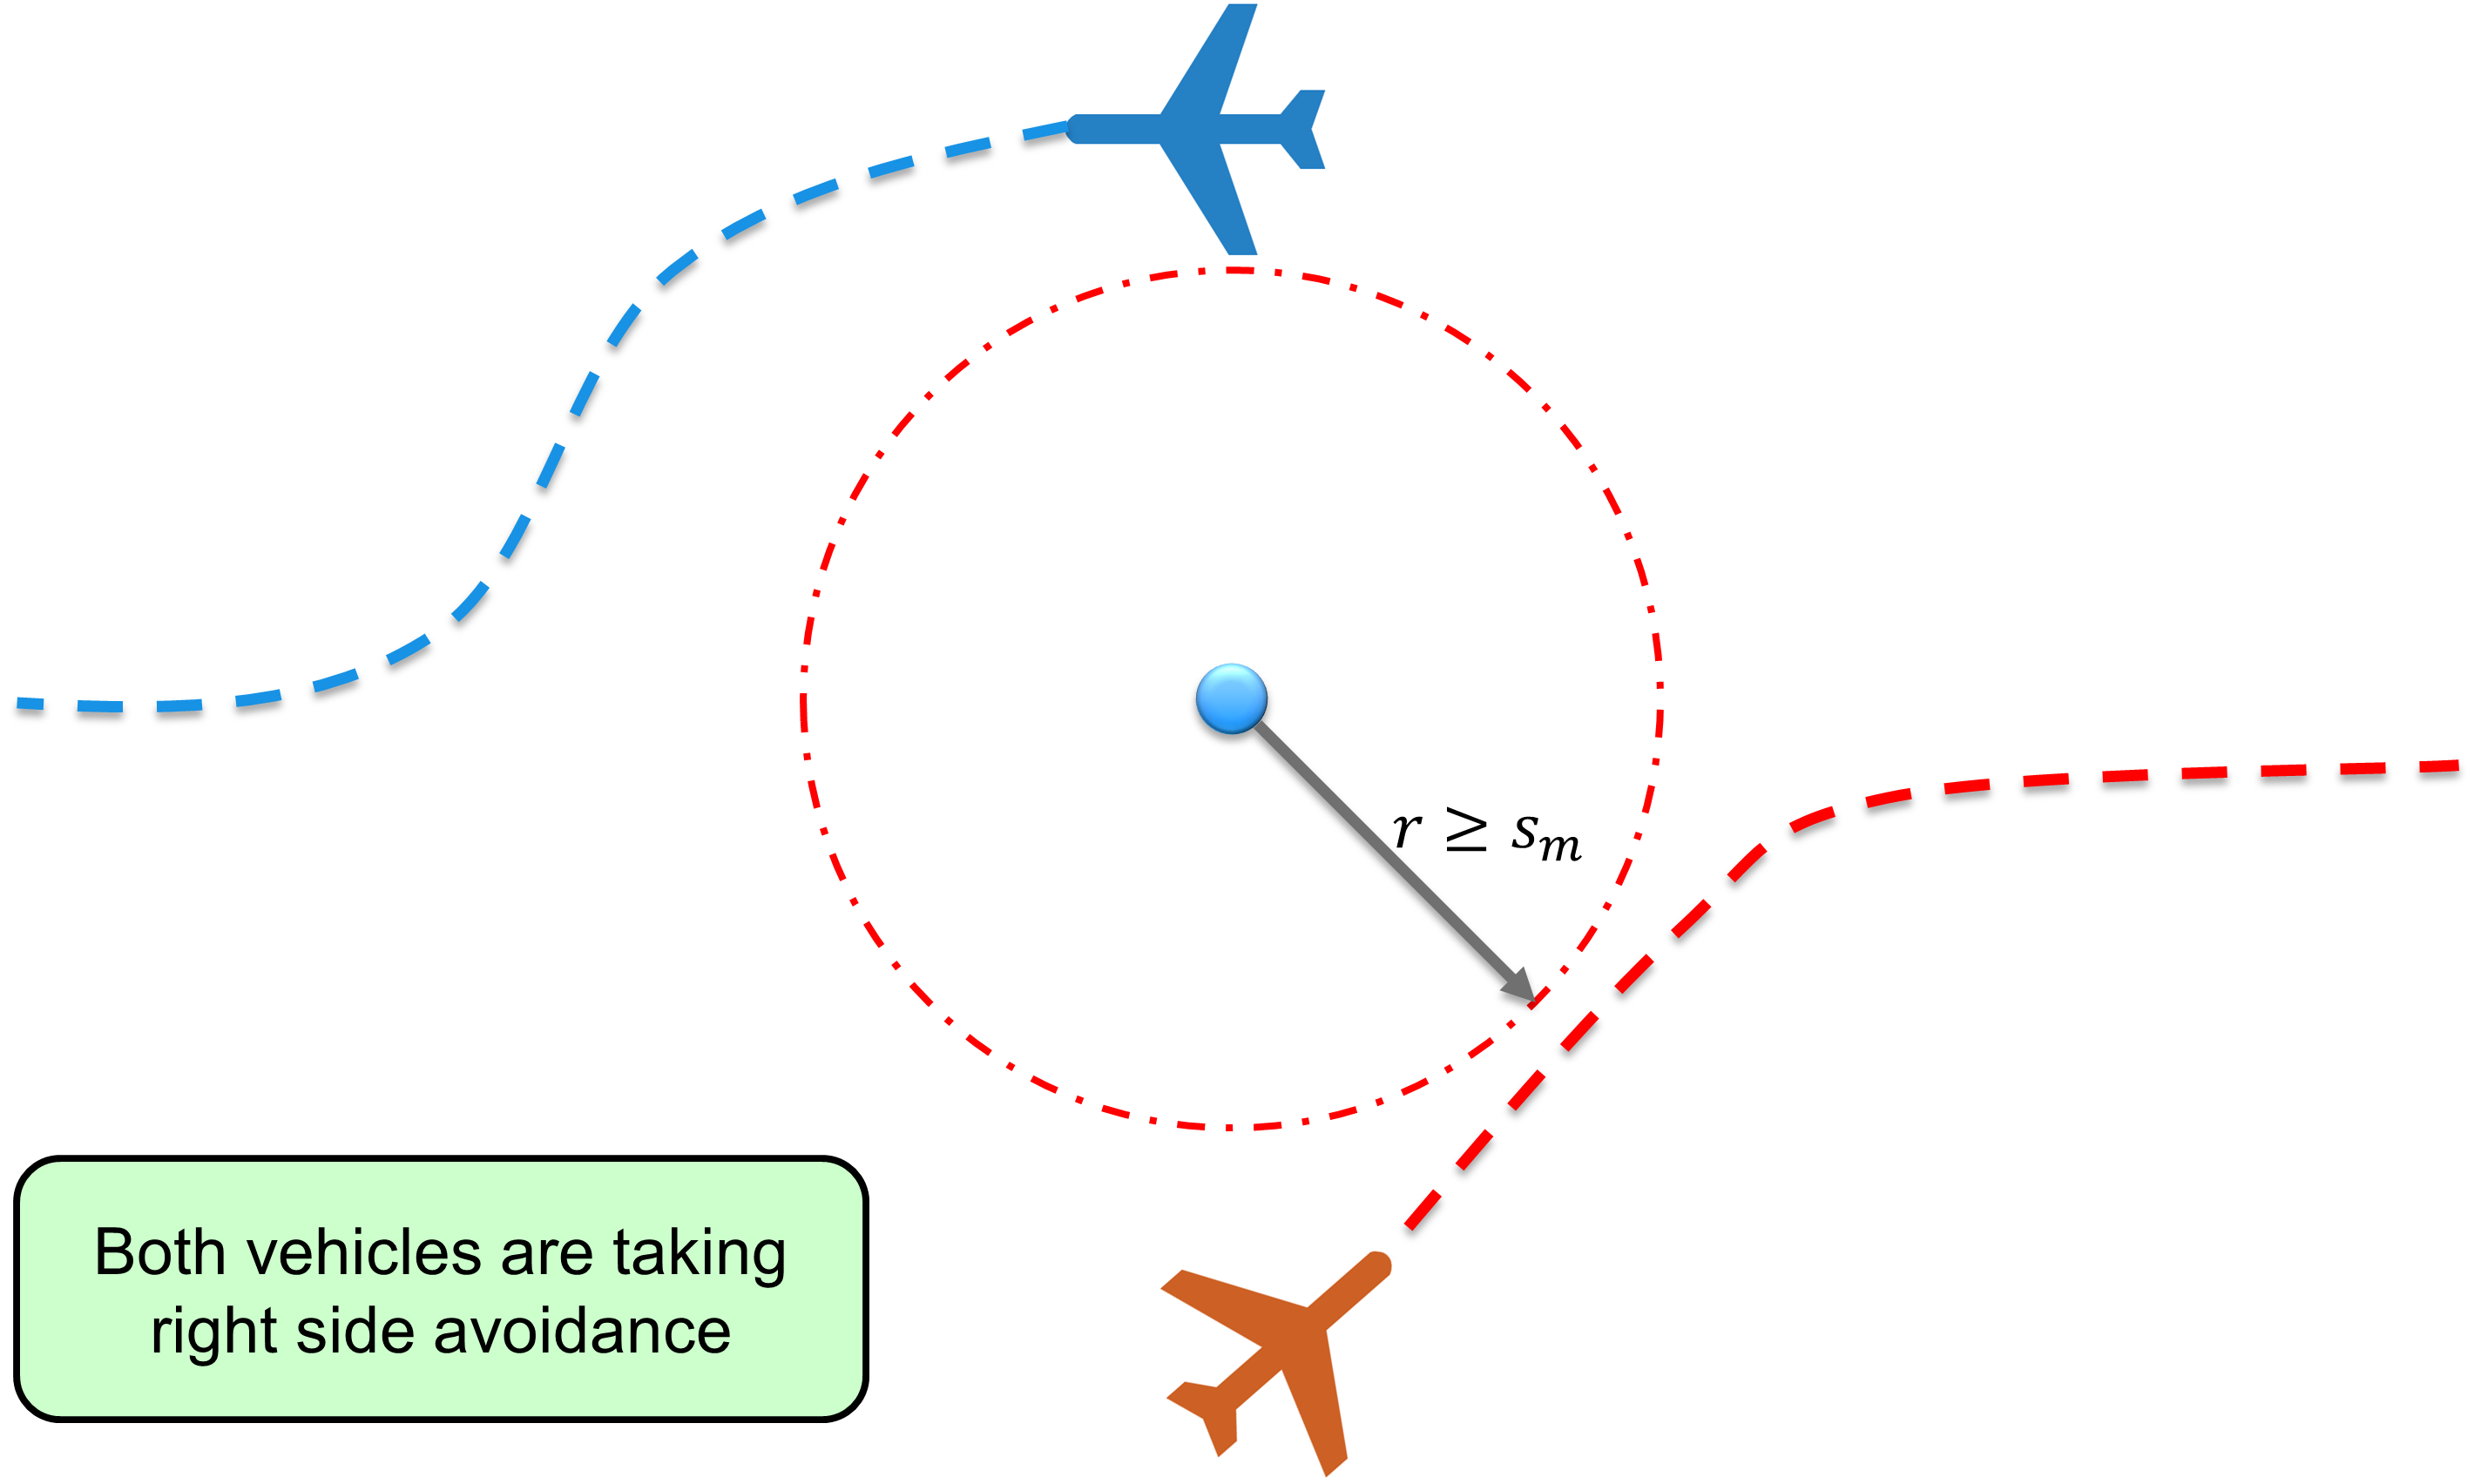
\includegraphics[width=0.9\linewidth,height=95pt,keepaspectratio]{\FIGDIR/RE009HeadOnApproach02} 
        \caption{Resolution/Closing.}
        \label{fig:HeadOnApproachTheoreticalResolution}
    \end{subfigure}
    \caption{Head-on approach detection/resolution/Closing}
    \label{fig:HeadOnApproachTheoretical}
\end{figure}

\paragraph{Triggering Events:} The \emph{head-on approach} (fig. \ref{fig:HeadOnApproachTheoretical}) \emph{triggering events} are the following:
\begin{enumerate}
    \item \emph{Detection} (fig. \ref{fig:HeadOnApproachTheoreticalDetection}) - the \emph{collision case} is open when \emph{collision point} with the respective angle of approach is detected. This must happen until the \emph{point of no return} is achieved. 
    
    \item \emph{Resolution} (fig. \ref{fig:HeadOnApproachTheoreticalResolution}) - the \emph{virtual} roundabout is enforced until the closing condition is met. 
    
    \item \emph{Closing} (fig. \ref{fig:HeadOnApproachTheoreticalResolution}) - based on the condition that all vehicles are heading away from \emph{collision point} and their mutual heading is neutral or opposite.
\end{enumerate} 

\paragraph{Virtual roundabout:} The \emph{flight levels} can be abstracted as the  \emph{virtual 2D surface}. The \emph{airspace attendants} are moving on virtual routes which can cross each other. The idea is to create virtual roundabout with enforced velocity to enable smooth collision avoidance.

\begin{enumerate}
    \item \emph{Center} - the center defined in \emph{airspace cluster} local coordinate system (flight level defining the horizontal placement).
    
    \item \emph{Diameter} - the minimal distance to \emph{center}, accounting the \emph{wake turbulence} and other phenomena. 
    
    \item \emph{Enforced velocity} - all attendants at \emph{virtual roundabout} keeps the same velocity. It helps to keep constant mutual distances.
\end{enumerate}



\subsection{Handling Converging Maneuver}\label{sec:handlingConvergingManuever}

\paragraph{Summary:} Two planned trajectories of the UAS are perpendicular, thus resulting in a protentional collision.  There is a need to define triggers for detection and resolution approach for autonomous UAS.  Rules for VFR/IFR modes in manned aviation are the base for the autonomous collision resolution.

\paragraph{Goal:} Identify \emph{required parameters} sufficient for automatic solution of \emph{Converging Maneuver}.

\paragraph{VFR:} The \emph{Visual Flight Rules} (VFR) are specified in annex 2 \cite{icaoAnnex2}. The rule is different from \emph{Head-on Approach} (sec. \ref{sec:handlingHeadOnApproach}) because multiple roles are depending on the relative aircraft position:
\begin{enumerate}
    \item \emph{Avoiding Aircraft} - there is an aircraft on the relative right side (blue). 
    \item \emph{Right Of the Way (ROA) Aircraft} - there is an aircraft on the relative left side (red). 
\end{enumerate}

The \emph{avoiding aircraft} should take the \emph{right of the way aircraft} from behind, with sufficient \emph{safety margin}, and return to original \emph{heading} afterward. The \emph{magnitude} of \emph{avoidance curve} must consider \emph{wake turbulence} and other impacts of \emph{avionic properties}.

\begin{note}
    This rule is applied only when both \emph{aircraft} belong to the same  \emph{maneuverability class} \cite{icaoAnnex2}.
\end{note}

\paragraph{IFR:} The \emph{Instrument Flight Rules} in annex 2. \cite{icaoAnnex2} and 11. \cite{icaoAnnex11} are defining \emph{converging maneuver} in detail.

The \emph{parameters} from a \emph{head-on approach} can be reused:
\begin{enumerate}
    \item $70^\circ$ $\le$ the \emph{Angle of Approach} $<$ $130^\circ$ - the minimal planar angle between aircraft position and expected collision point is in the interval $[70^\circ , 130^\circ[$.
    
    \item\emph{Minimal detection range} - given as $turning Radius + safety Margin$, while \emph{safety margin} is accounting all impact factors. 
    
    \item\emph{Safety margin} - during avoidance all aircraft keeps mutual distance at least on the value of \emph{Safety Margin}.
\end{enumerate}

\begin{note}
The lesser \emph{angle of approach} induces stronger wake turbulence impact on avoiding aircraft. This results in an increase of \emph{safety margin}. 

The \emph{wake turbulence} is represented as a droplet at the back of the plane. \emph{Wake turbulence range} can be calculated based on wake turbulence cone.
\end{note}

\begin{figure}[H]
	\centering
    \begin{subfigure}{0.32\textwidth}
    	\centering
        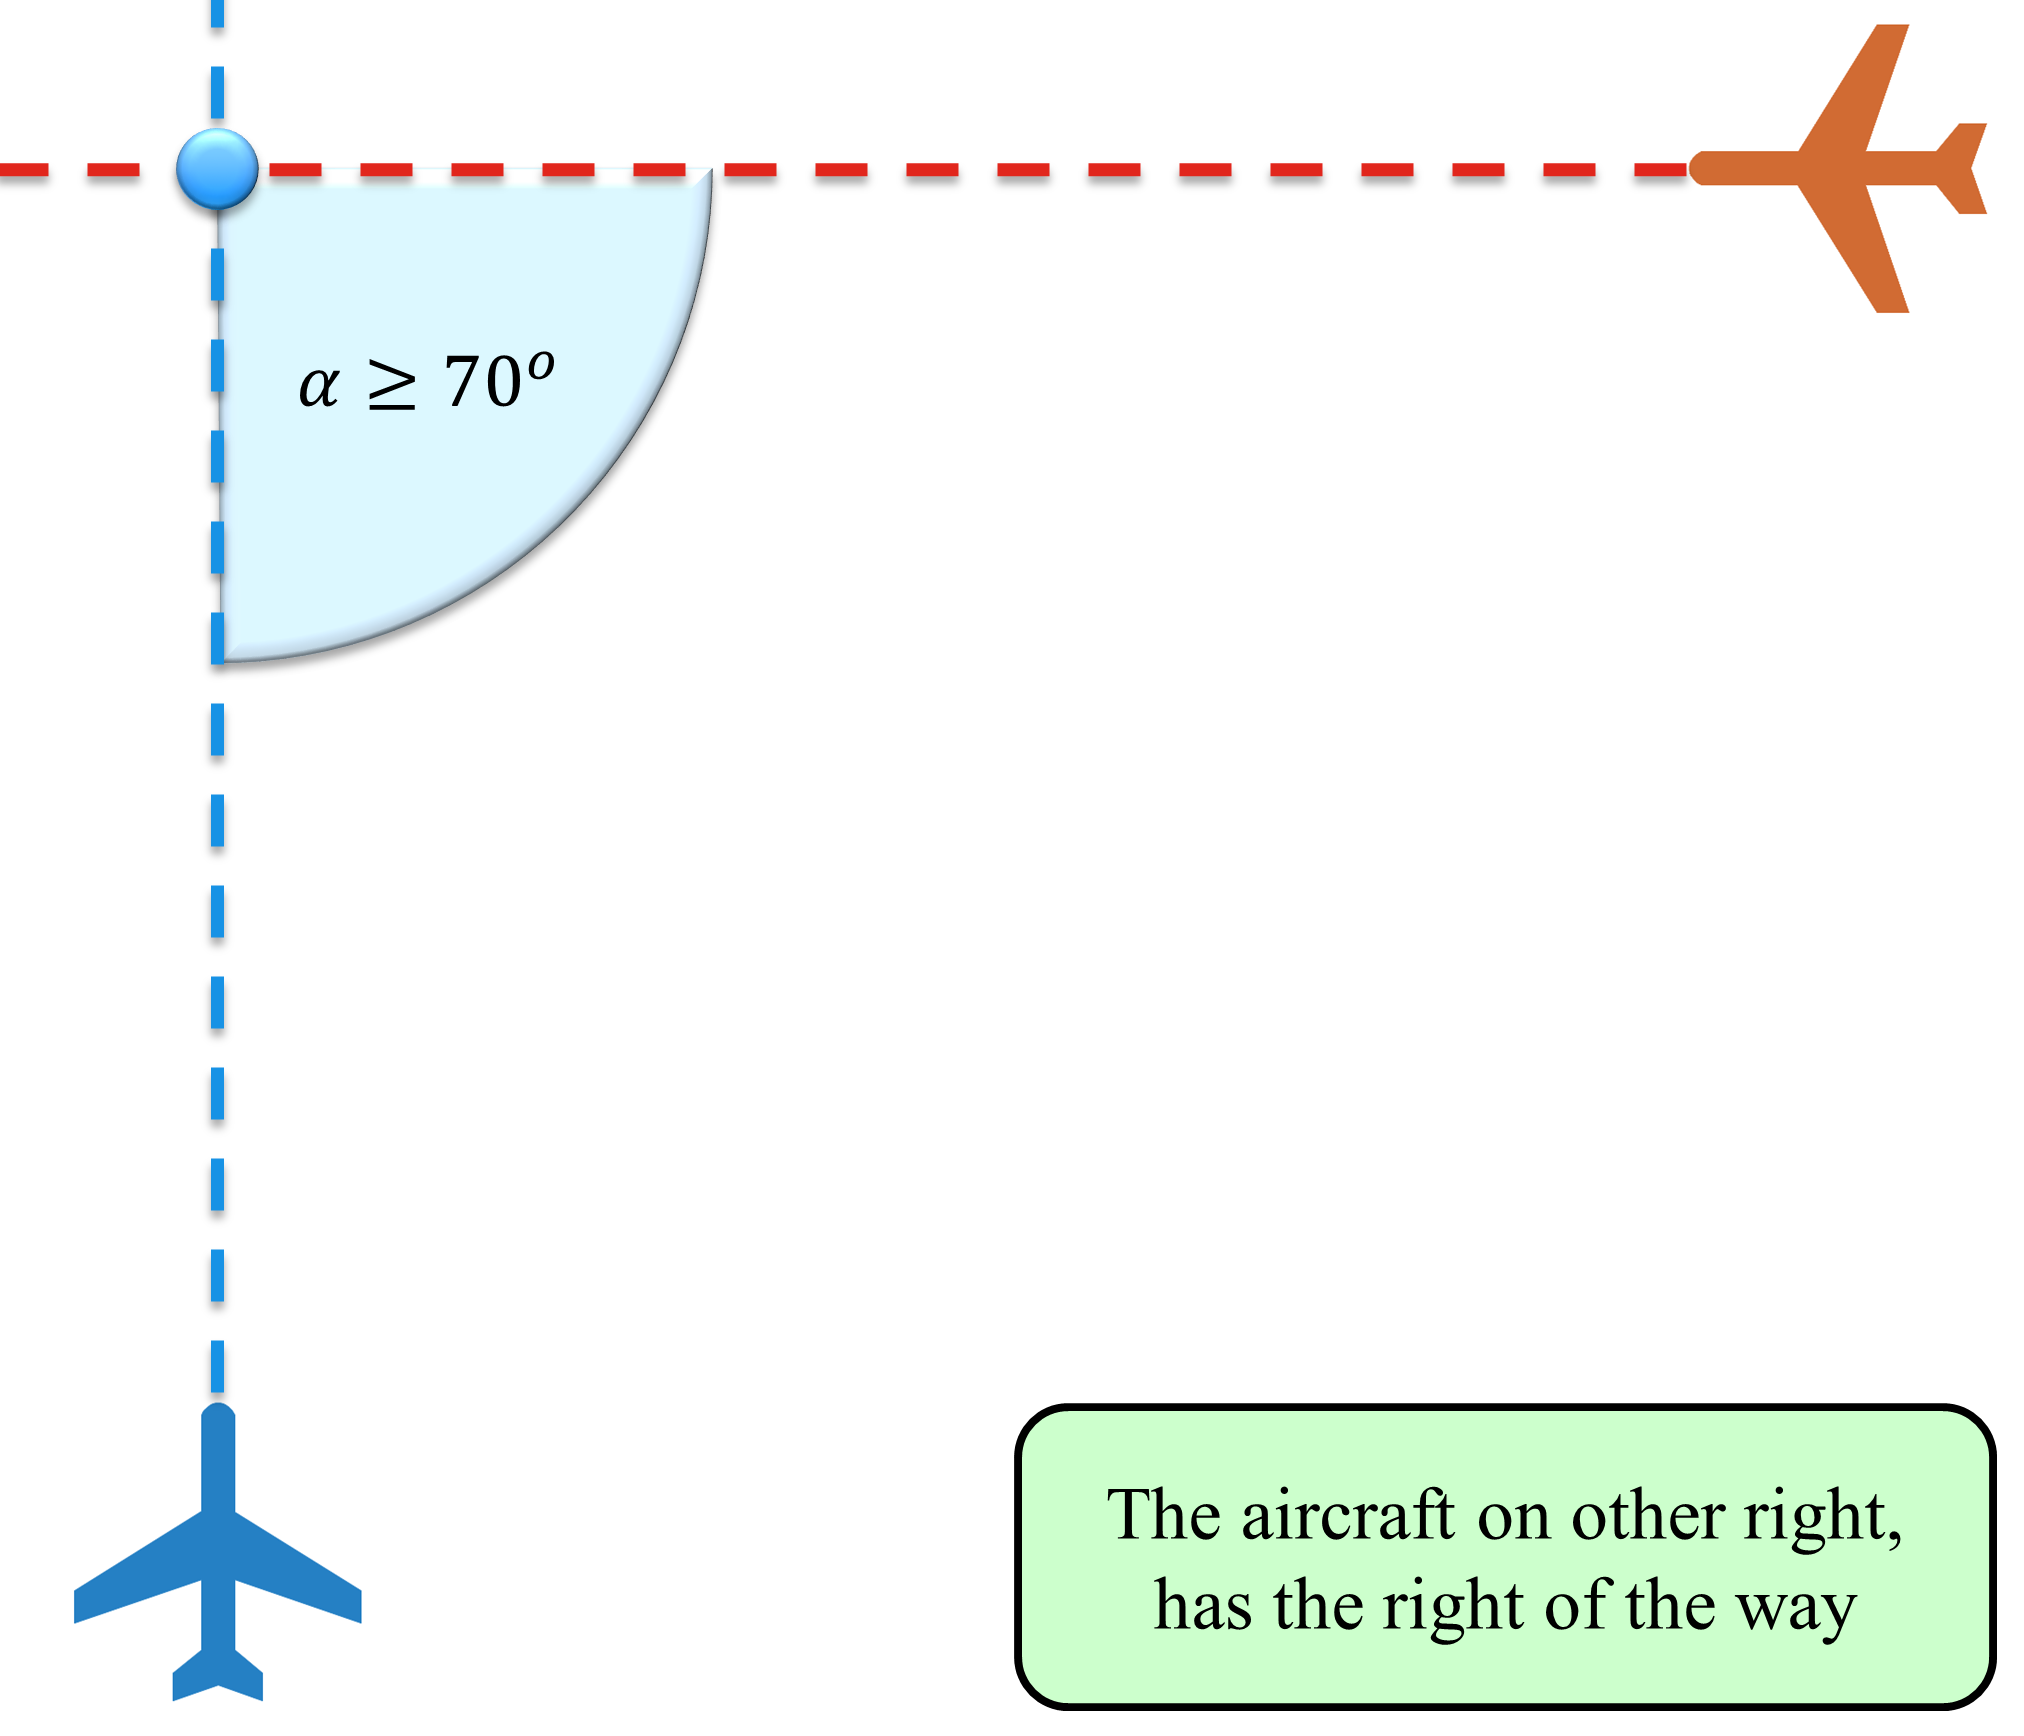
\includegraphics[width=0.9\linewidth,height=105pt,keepaspectratio]{\FIGDIR/RE005ConvergingManeuver01} 
        \caption{Detection.}
        \label{fig:ConvergingManeuverTheoreticalDetection}
    \end{subfigure}
    \begin{subfigure}{0.32\textwidth}
        \centering
        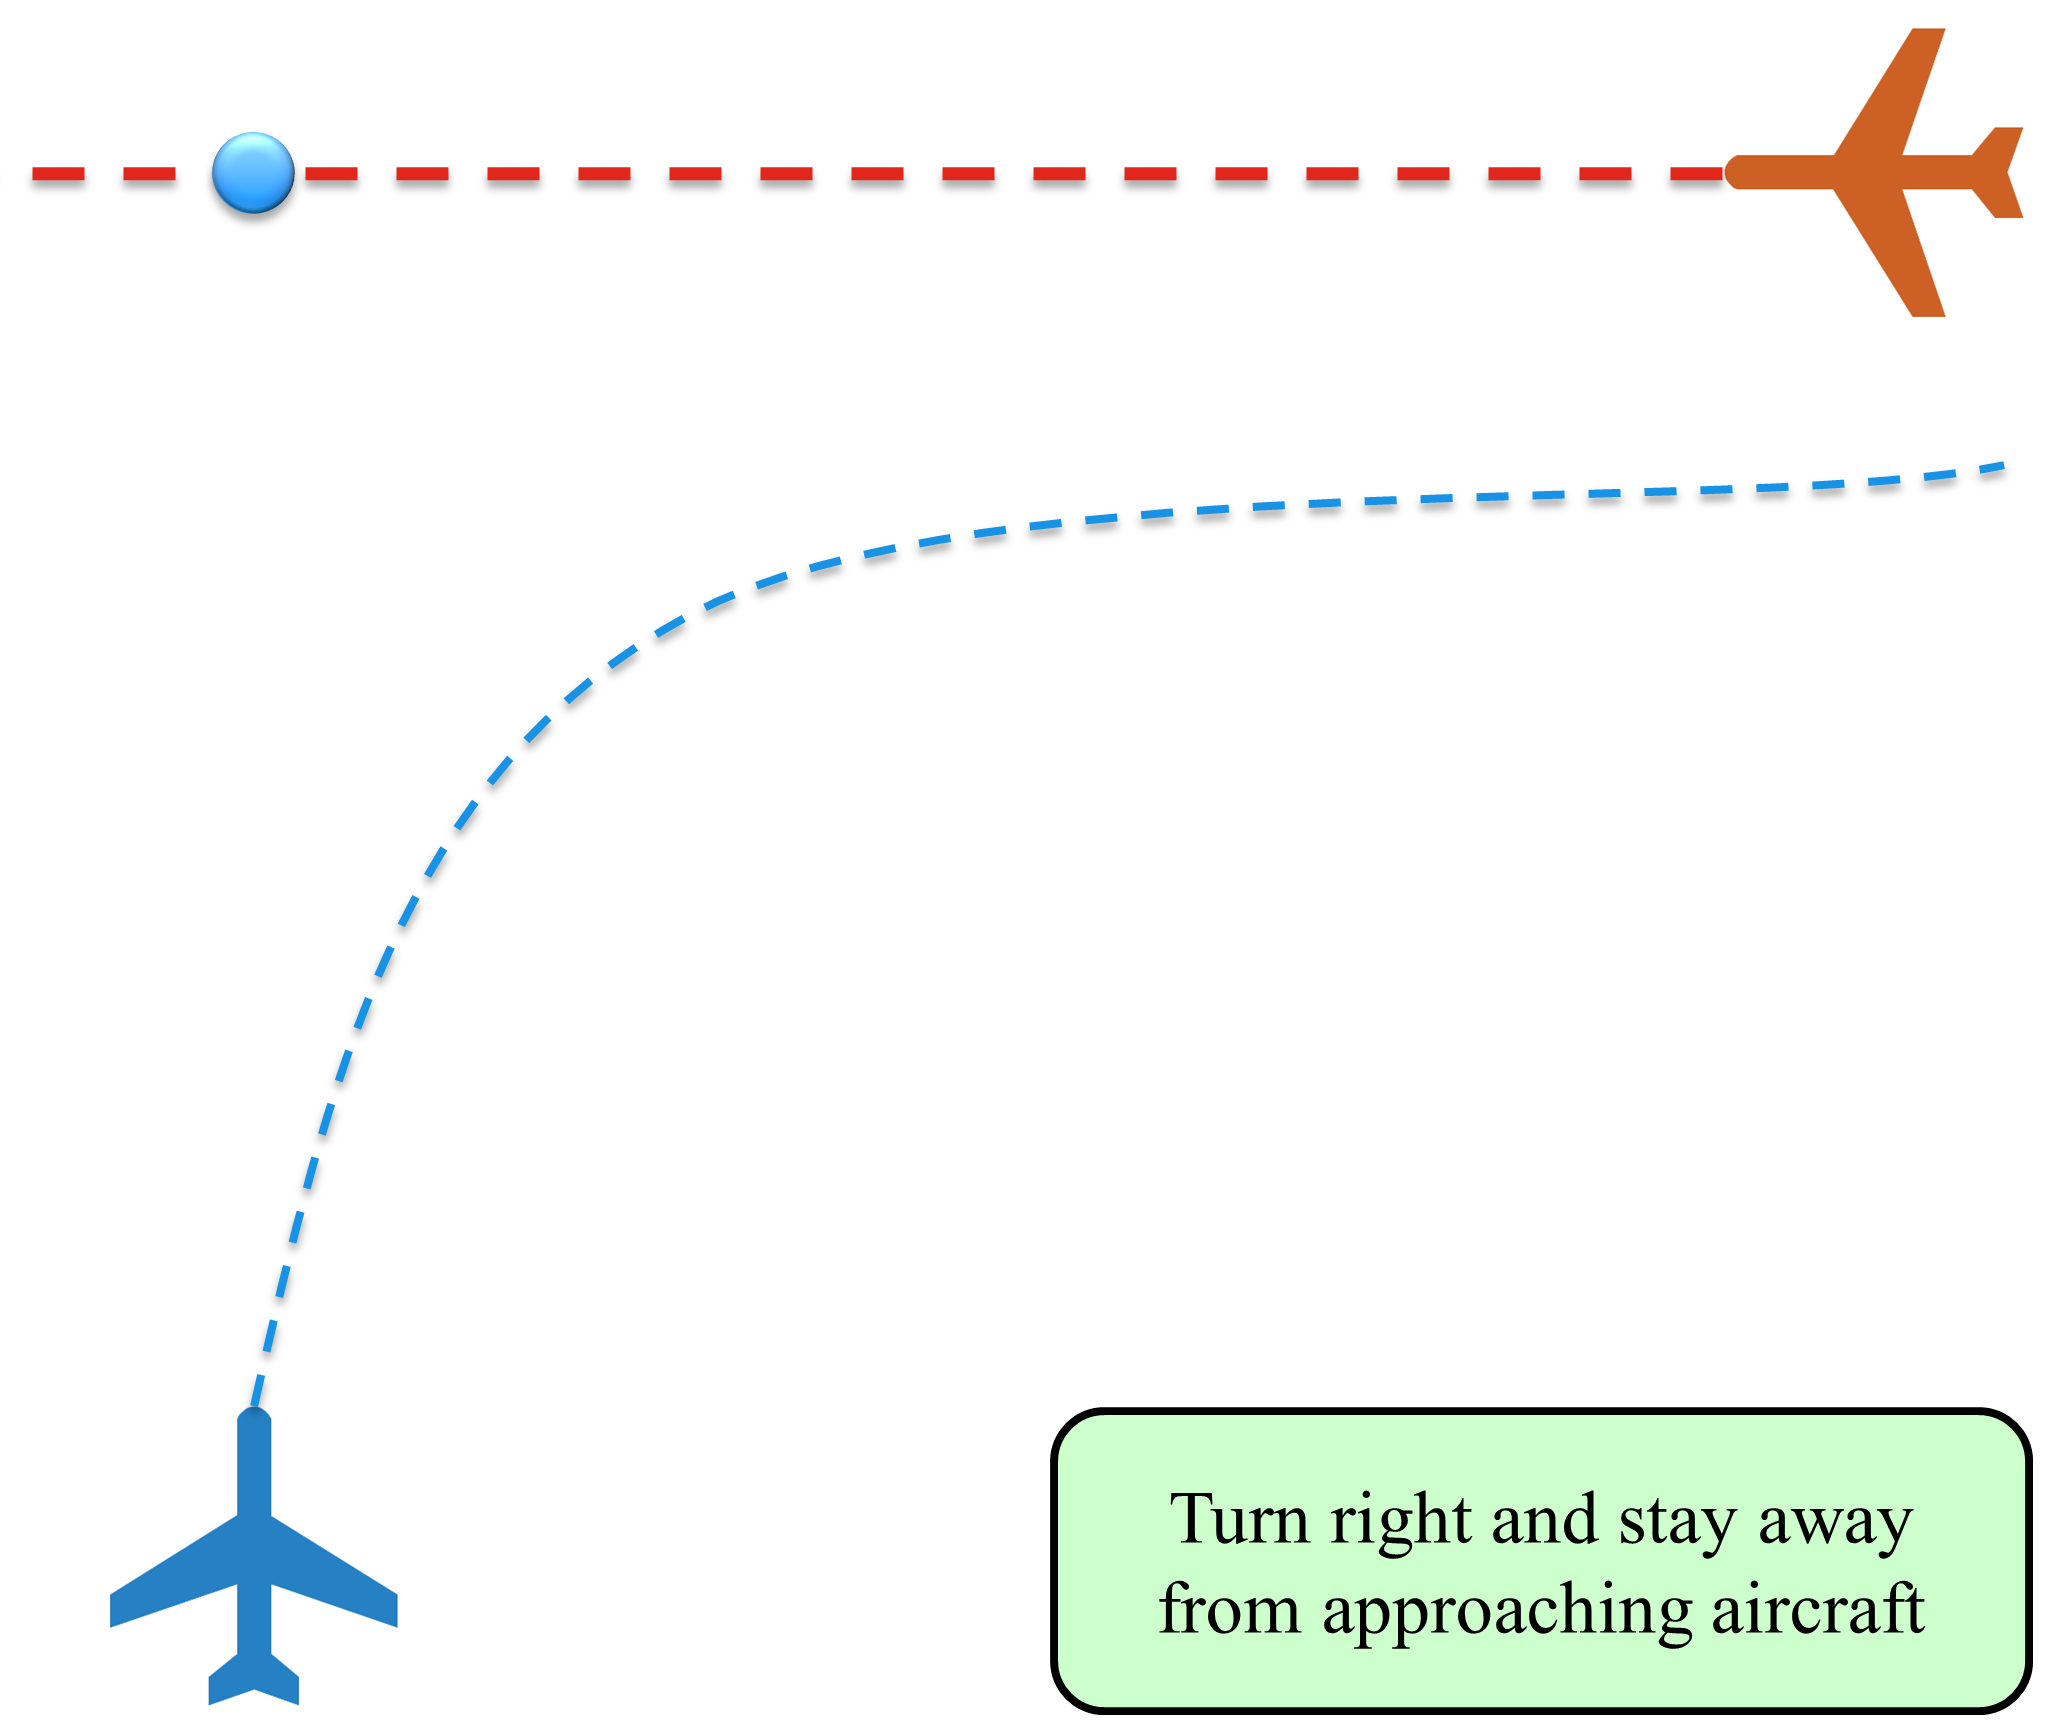
\includegraphics[width=0.9\linewidth,height=105pt,keepaspectratio]{\FIGDIR/RE006ConvergingManuever02} 
        \caption{Resolution.}
        \label{fig:ConvergingManeuverTheoreticalResolution}
    \end{subfigure}
    \begin{subfigure}{0.32\textwidth}
        \centering
        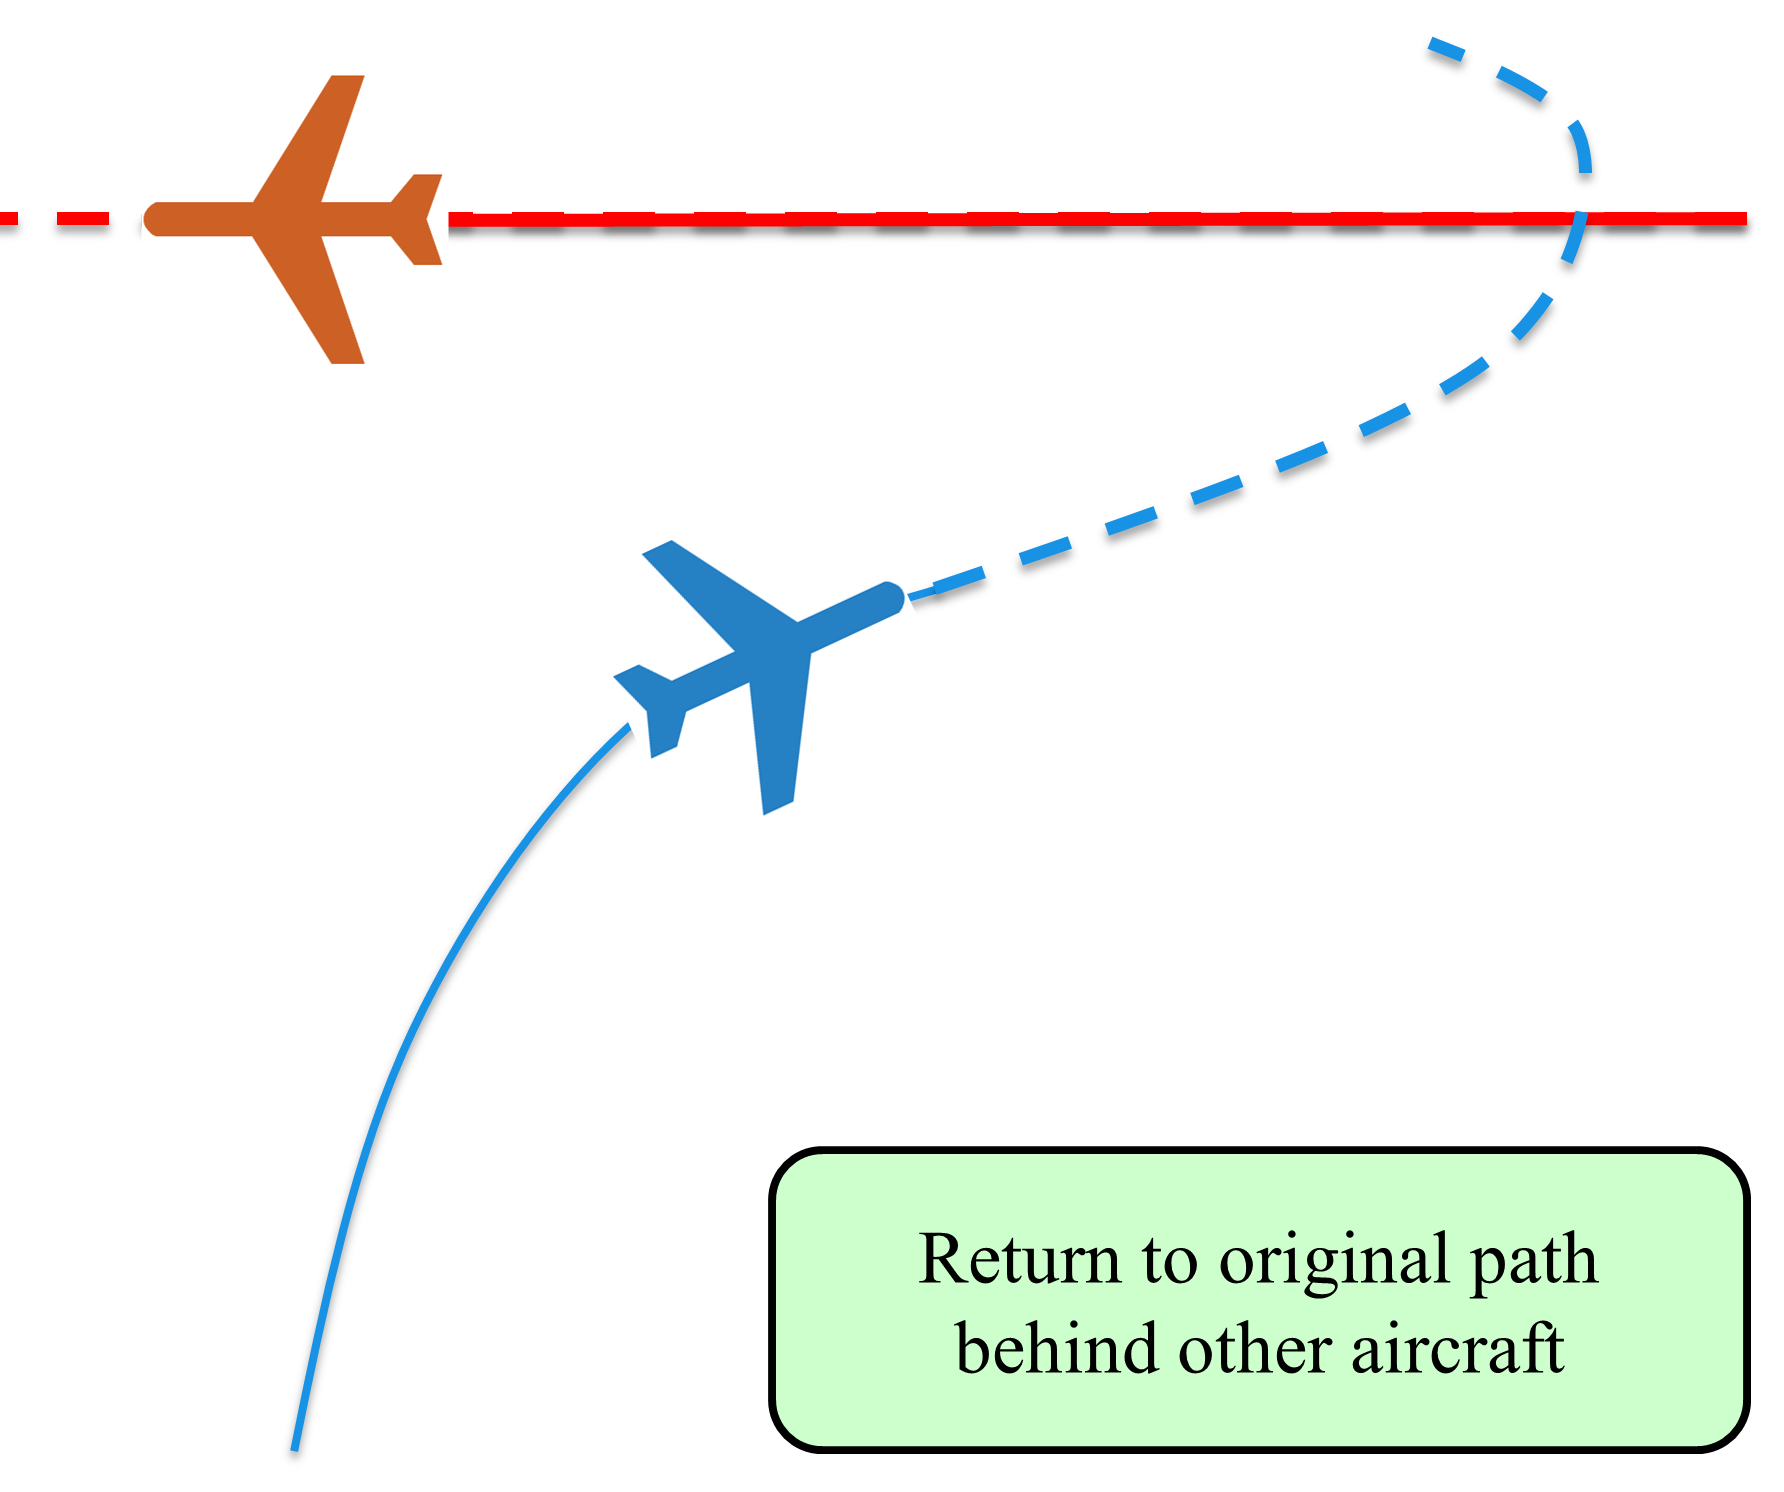
\includegraphics[width=0.9\linewidth,height=105pt,keepaspectratio]{\FIGDIR/RE007ConvergingManuever03} 
        \caption{Closing}
        \label{fig:ConvergingManeuverTheoreticalClosure}
    \end{subfigure}
    \caption{Converging maneuver Detection/Resolution/Closing}
    \label{fig:ConvergingManeuverTheoretical}
\end{figure}

\paragraph{Triggering Events:} The \emph{converging maneuver} (fig. \ref{fig:ConvergingManeuverTheoretical}) \emph{triggering events} are the following:

\begin{enumerate}
    \item \emph{Detection} (fig. \ref{fig:ConvergingManeuverTheoreticalDetection}) -  The \emph{avoiding airplane} (blue) detects \emph{collision point} (blue circle) which satisfy the \emph{converging maneuver conditions}. The distance between \emph{aircraft position} and \emph{collision point} is lesser than the \emph{detection range}.
    
    \item \emph{Resolution} (fig. \ref{fig:ConvergingManeuverTheoreticalResolution}) - the \emph{Right Of the Way aircraft} (red) stays at the original course. The \emph{avoiding aircraft} (blue) follows the \emph{parallel} to another \emph{plane}. The distance of \emph{avoiding plane} to \emph{other plane trajectory} is greater or equal to \emph{safety margin}.
    
    \item \emph{Closing} (fig. \ref{fig:ConvergingManeuverTheoreticalClosure}) - when both planes have an opposite heading, and they miss each other the converging maneuver can be closed. The \emph{avoiding airplane} will return to \emph{original trajectory}  while keeping the distance from \emph{another plane} (red) at greater or equal to \emph{safety margin}.
\end{enumerate}


\subsection{Handling Overtake Maneuver}\label{sec:handlingOvertakeManuever}

\paragraph{Summary:} Two UAS are on the same airway, flying in the same direction. The slower UAS is in front of the faster UAS. The slower UAS has the right of way, and the faster UAS needs to make an overtake. There is a need to define triggers for detection and resolution approach for autonomous UAS.  Rules for VFR/IFR modes in manned aviation are the base for the autonomous collision resolution.

\paragraph{Goal:} Identify \emph{required parameters} sufficient for automatic solution of \emph{Overtake Maneuver}

\paragraph{VFR:} The \emph{Visual Flight Rules} (VFR) are specified in annex 2 \cite{icaoAnnex2}. The rule states that faster air traffic attendant may overtake slower one, from right side keeping sufficient distance (\emph{safety margin}). There are two forced roles:

\begin{enumerate}
    \item \emph{Overtaking} - faster aircraft with similar heading cruising in similar altitude than \emph{overtaken} (blue). It is expected that \emph{faster aircraft} has maneuvering capability to avoid slower aircraft.
    
    \item \emph{Overtaken} - slower aircraft which keeps the \emph{Right of the way}
\end{enumerate}

\begin{note}
    This rule is applied only when both aircraft have the same maneuverability class \cite{icaoAnnex2}. The overtake is considered \emph{borderline emergency maneuver} in controlled airspace because the aircraft tend to keep similar velocity in similar cruising altitude. The overtake is usual in \emph{non-controlled airspace}.
\end{note}

\begin{figure}[H]
	\centering
    \begin{subfigure}{0.32\textwidth}
        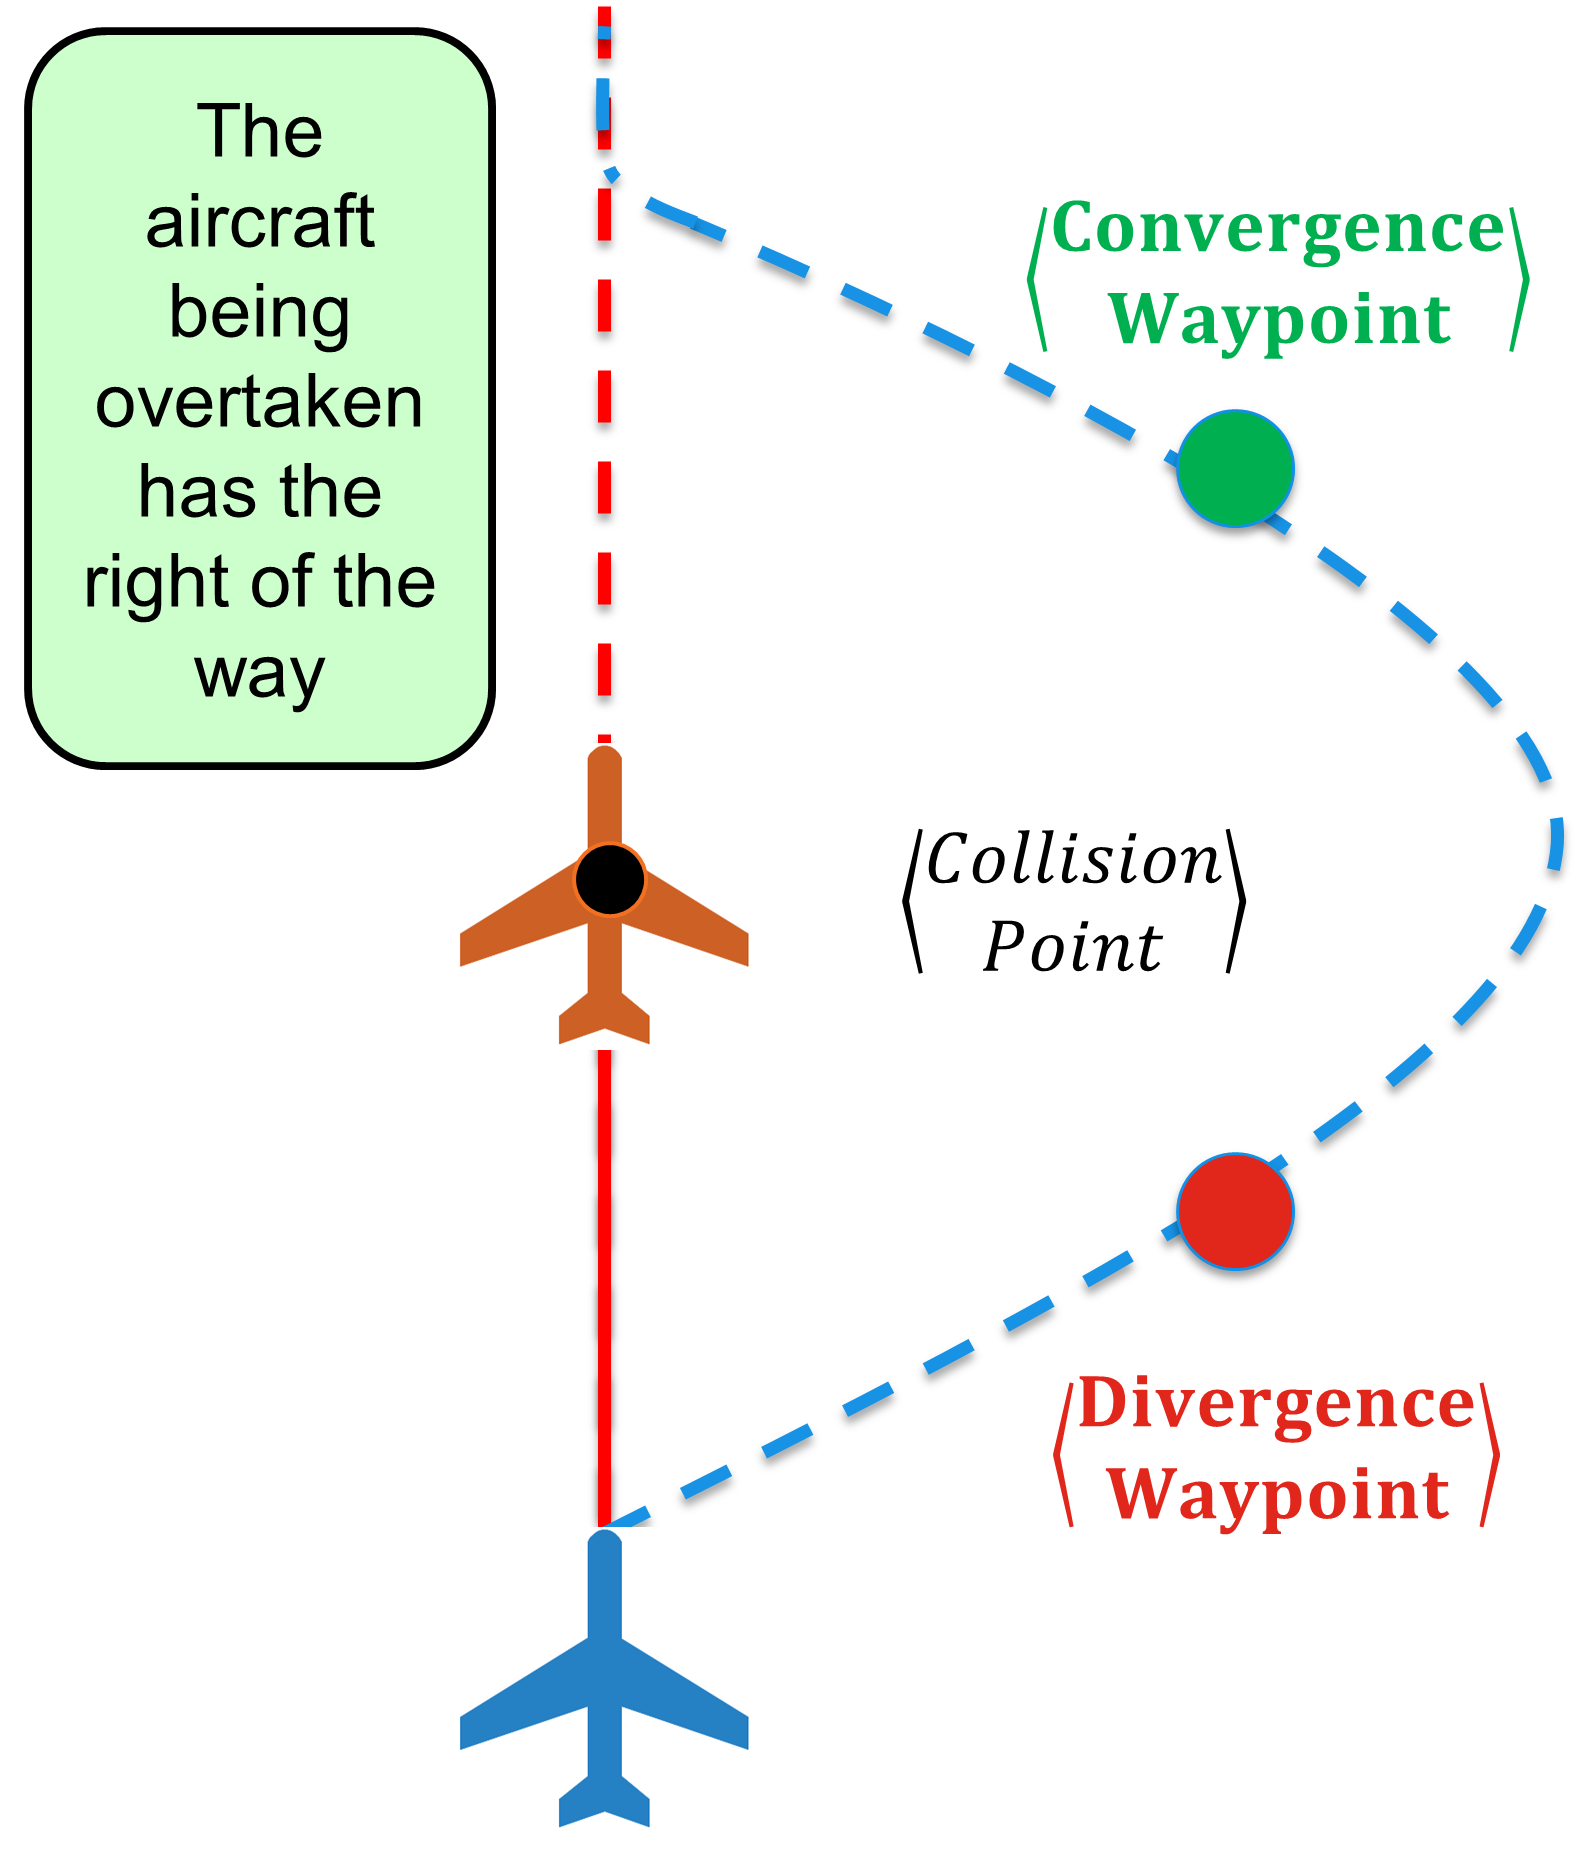
\includegraphics[width=0.9\linewidth,height=142pt,keepaspectratio]{\FIGDIR/RE010OvertakeMAnuever01} 
        \caption{Detection.}
        \label{fig:OvertakeManeuverTheoreticalDetection}
    \end{subfigure}
    \begin{subfigure}{0.32\textwidth}
        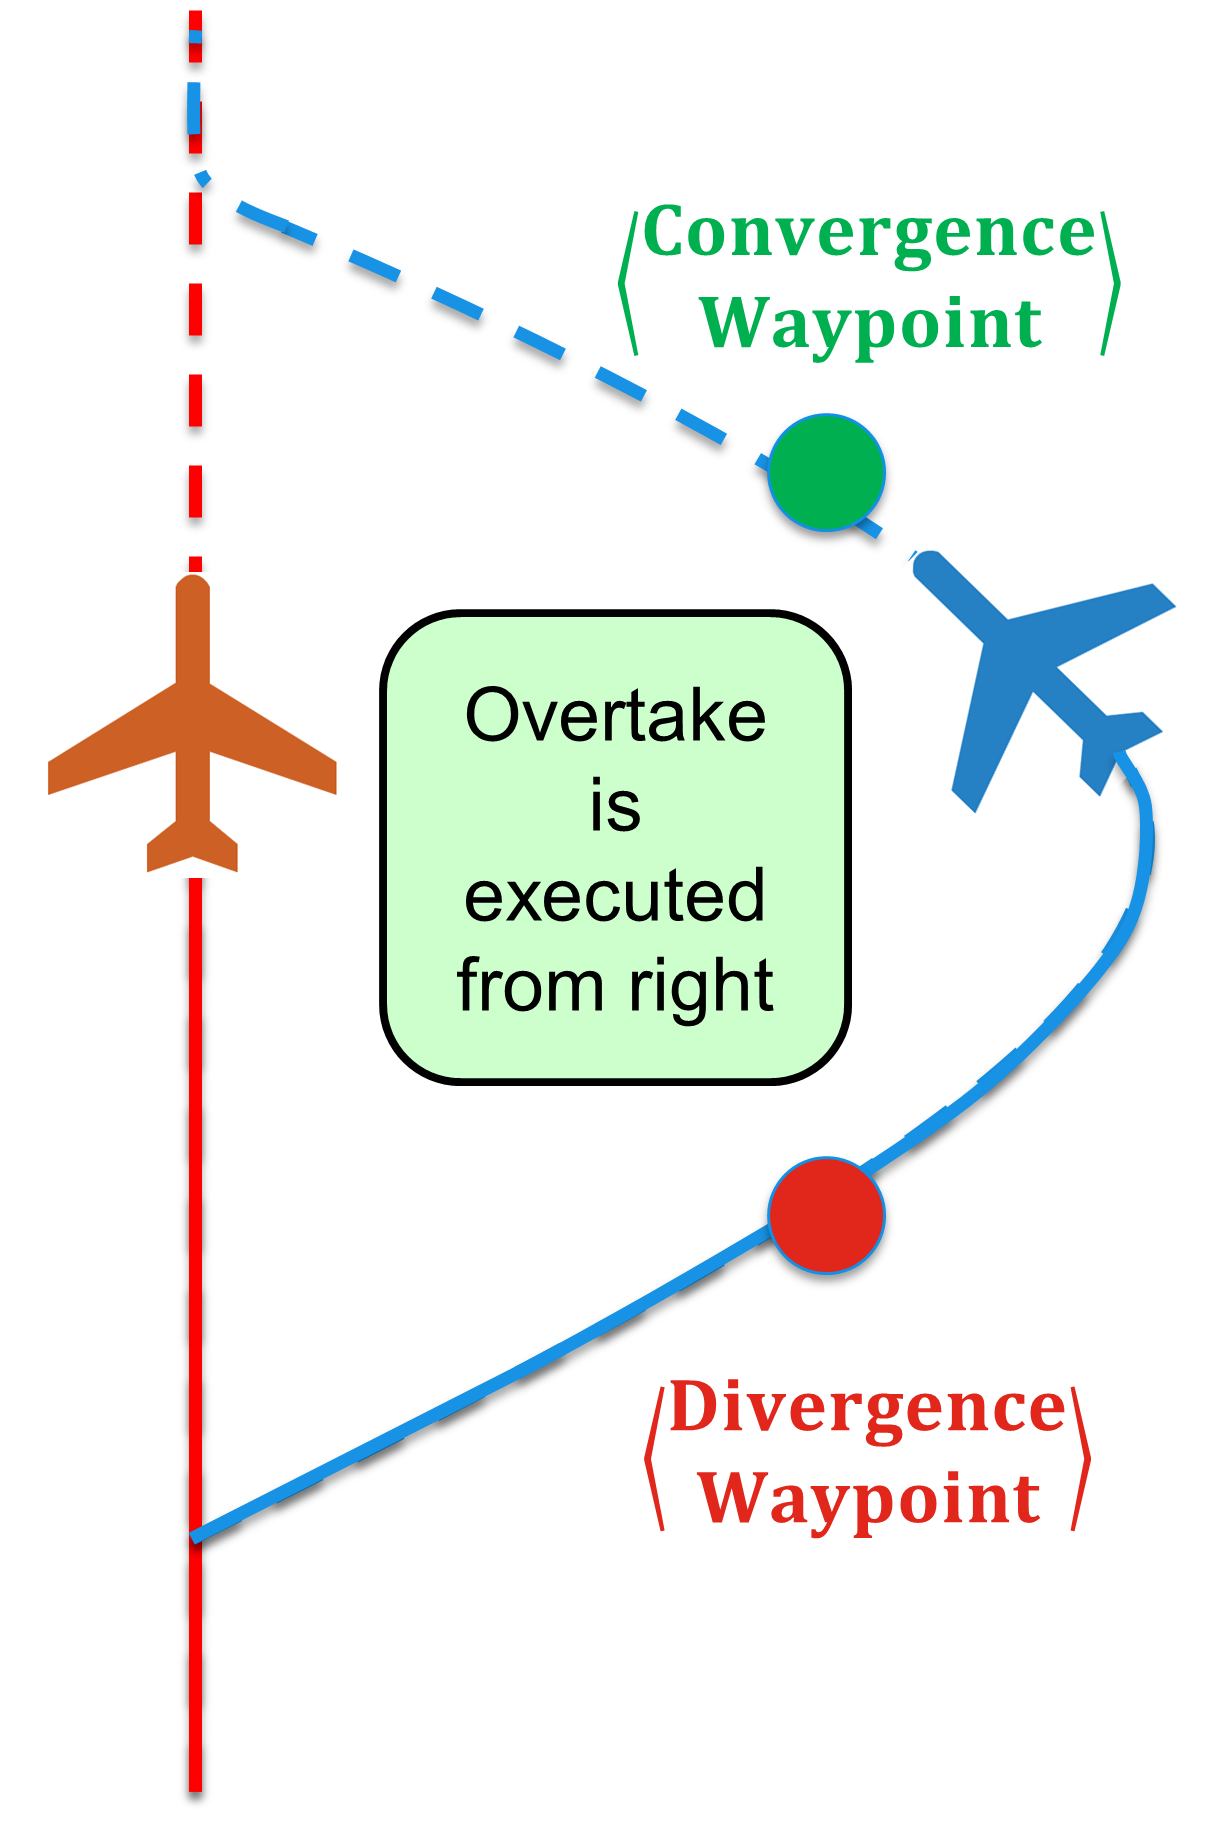
\includegraphics[width=0.9\linewidth,height=142pt,keepaspectratio]{\FIGDIR/RE011OvertakeMAnuever02} 
        \caption{Resolution.}
        \label{fig:OvertakeManeuverTheoreticalResolution}
    \end{subfigure}
    \begin{subfigure}{0.32\textwidth}
        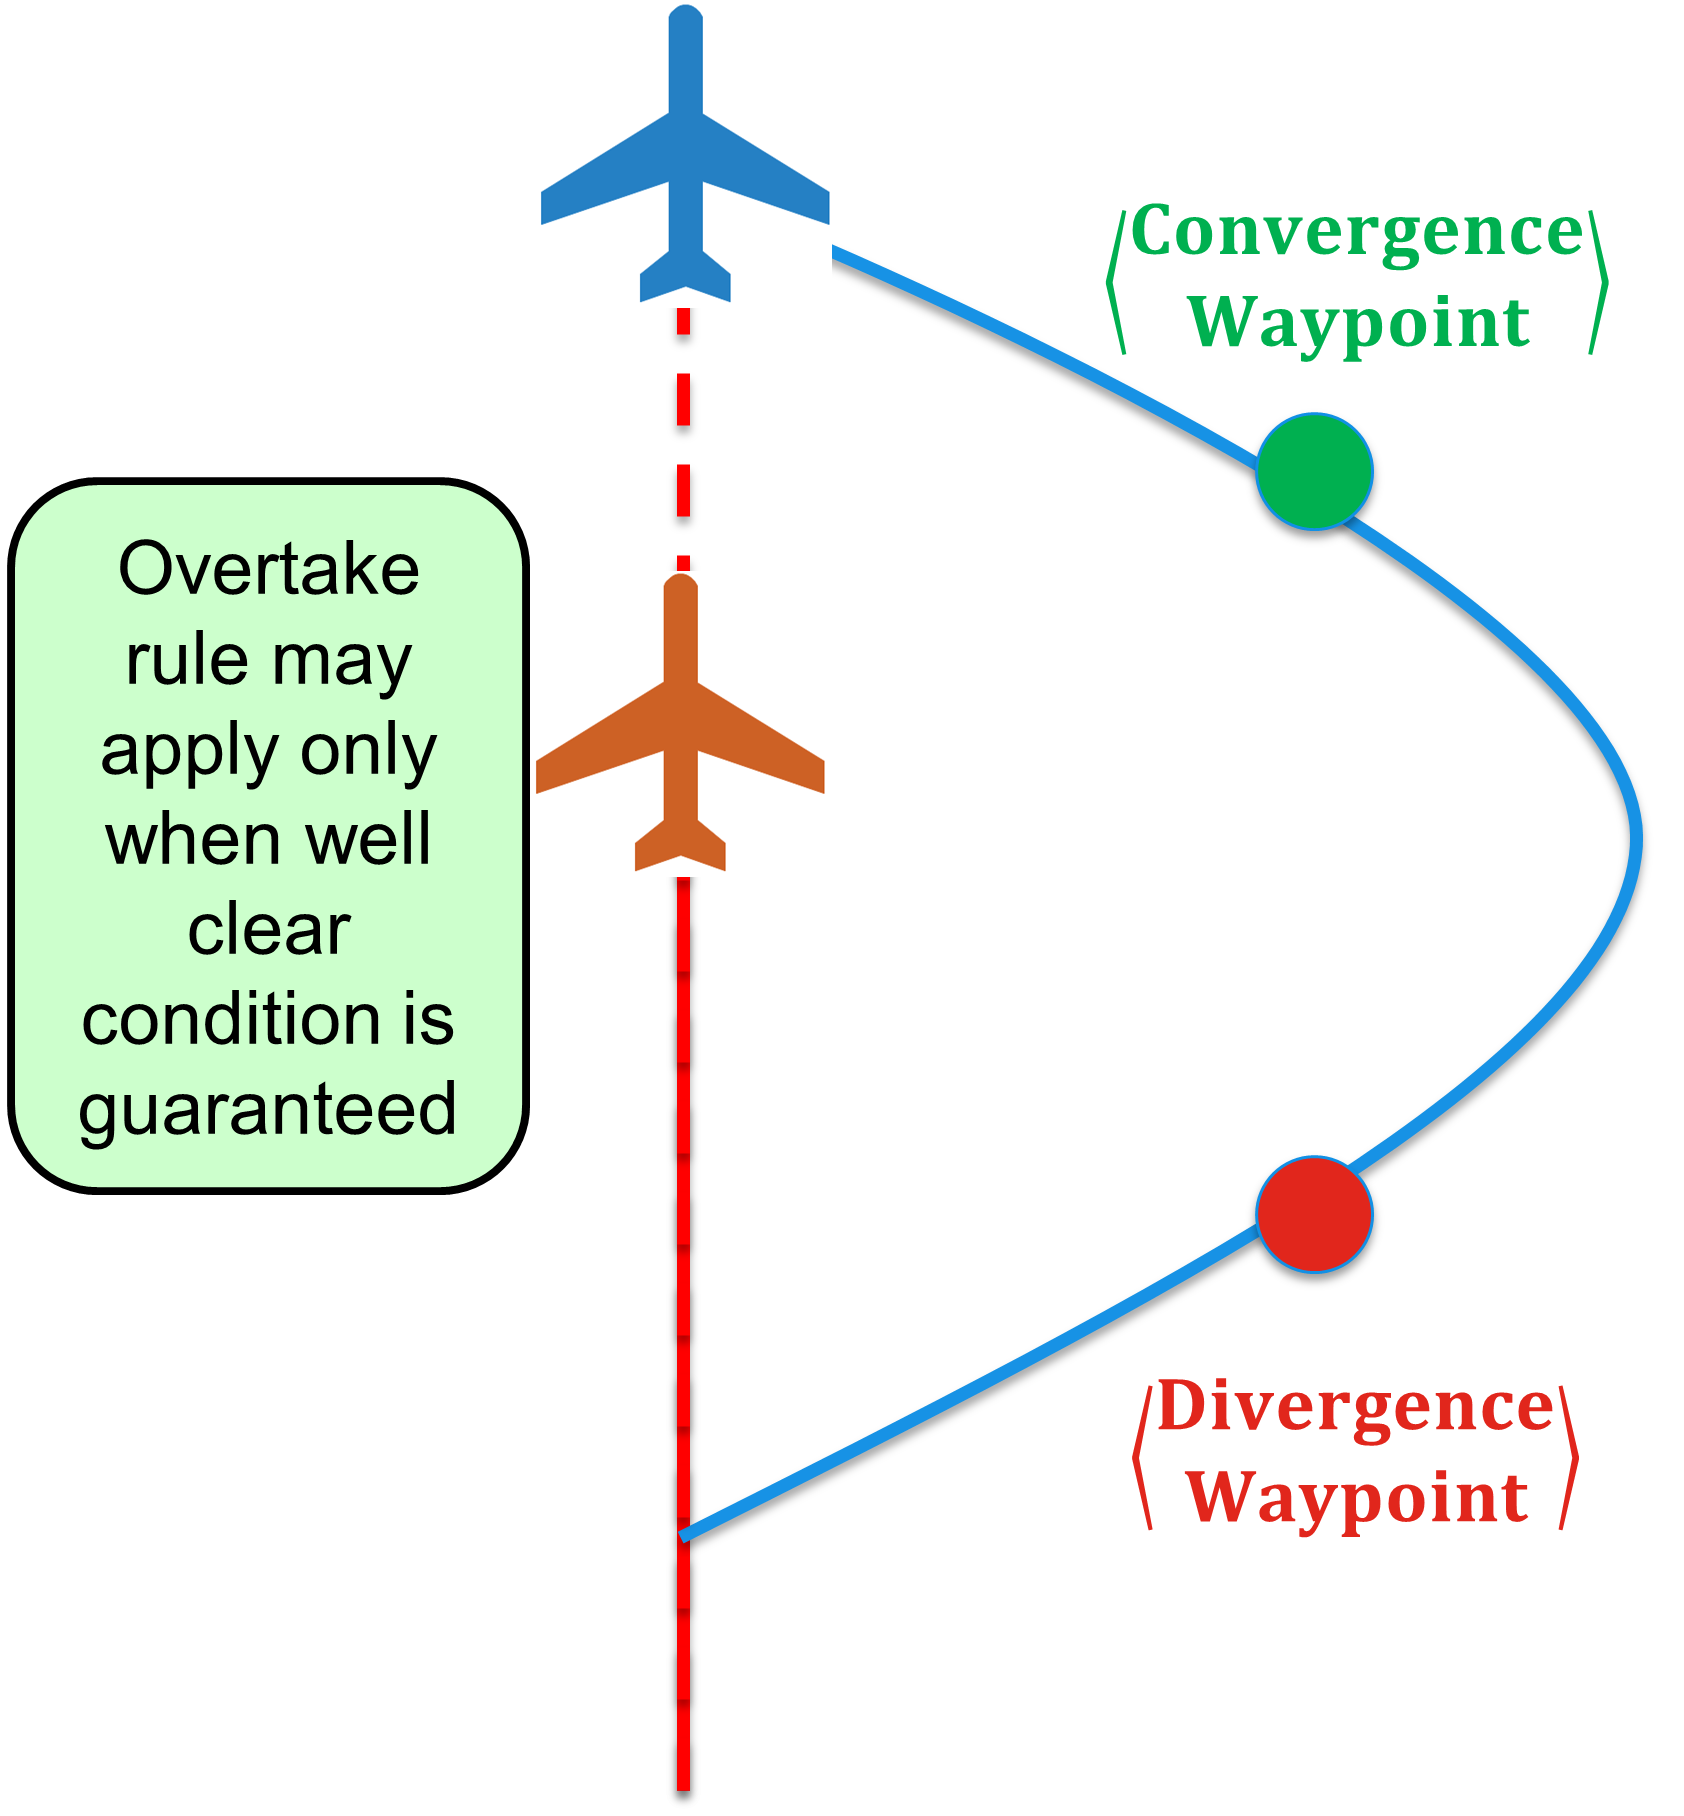
\includegraphics[width=0.9\linewidth,height=142pt,keepaspectratio]{\FIGDIR/RE012OvertakeMAnuever03} 
        \caption{Closing.}
        \label{fig:OvertakeManeuverTheoreticalClosure}
    \end{subfigure}
    \caption{Overtake maneuver Detection/Resolution/Closing}
    \label{fig:OvertakeManeuverTheoretical}
\end{figure}

\paragraph{IFR:} The \emph{Instrument Fight Rules} in annex 2. \cite{icaoAnnex2} and 11. \cite{icaoAnnex11} are defining the converging manual in detail:

\begin{enumerate}
    \item 0$^\circ \le$ the \emph{Angle of Approach} $<$ 130$^\circ$ - the minimal planar angle between aircraft position and expected collision point is in the interval $[0^\circ,70^\circ[$
    
    \item \emph{Minimal Detection Range} - given as $2 \times  reaction Time \times speed Difference$. 
    
    \item \emph{Safety Margin} - during avoidance the overtaking aircraft keeps the minimal distance of \emph{wake turbulence} of overtaken aircraft in own flight altitude. 
\end{enumerate}

\begin{note}
    The \emph{Safety Margin} is sufficiently small because speed difference is usually much lesser than in case of  \emph{Head-on approach}. The \emph{Wake turbulence} can be avoided completely by taking the higher altitude level than overtaken aircraft.
\end{note}


\paragraph{Triggering events:}
\begin{enumerate}
    \item \emph{Detection} (fig. \ref{fig:OvertakeManeuverTheoreticalDetection}) - occurs when the distance between \emph{overtaking} (blue) and overtaken (red) is approaching \emph{minimal detection range} or double of \emph{safety margin}. If the performance of \emph{overtaking aircraft} (blue) allows taking \emph{sharp right side to overtake} the \emph{Maneuver starts}, otherwise \emph{overtaking aircraft} (blue slows down) and keeps at least \emph{safety margin distance} to avoid \emph{wake turbulence}.
    
    \item \emph{Resolution} (fig. \ref{fig:OvertakeManeuverTheoreticalResolution}) - \emph{overtaken} (red) is keeping same heading and \emph{speed} during overtake maneuver. The \emph{overtaking} (blue) projects two waypoints: \emph{Divergence} and \emph{Convergence} keeping the required separation minimum during overtake. Then the \emph{overtaking} (blue) diverges heading to \emph{Divergence waypoint}. When the \emph{Divergence waypoint} is reached by \emph{overtaking} (blue) aircraft, it changes to \emph{original heading}.
    
    \item \emph{Closing} (fig. \ref{fig:OvertakeManeuverTheoreticalClosure}) - the \emph{closing} of \emph{Overtake} starts when \emph{overtaking} aircraft (blue) have sufficient lead over \emph{overtaken} aircraft (red). The \emph{overtaking} aircraft (blue) can safely change the heading to the original waypoint.
\end{enumerate}


\paragraph{Constant Cruising Speed:} Most of the traffic attendants at same flight level have similar (close to constant) cruising speed. Lower flight levels are for slower turbo-prop planes, and higher altitudes are for jet planes. It is stated that this principle will persist even when UAS will be integrated \cite{bayen2005langrangian,kopardekar2002dynamic,helme1992optimization} in multiple air-traffic models.



		\subsection{\secState{R}Position Notification}\label{sec:positionNotification}

\paragraph{Motivation:} The \emph{position notification} (tab. \ref{tab:positionNotification}) is designed for further \emph{collision case resolution} (sec. \ref{sec:collisionCase}). It is similar to ADS-B\footnote{ADS-B versions and message containment: \url{https://mode-s.org/decode/adsb/version.html}.} message information. 


The main purpose is to broadcast the \emph{position notification} in \emph{controlled aerospace}. The broadcast for \emph{non-controlled} airspace needs to contain \emph{intruder properties}, \emph{preferred separation mode} and \emph{near-miss margin}.

\paragraph{Position:} The position is defined in \emph{Global Coordinate System} using GPS for latitude and longitude. The barometric altitude is required for controlled airspace, preferred for non-controlled airspace.

\paragraph{Heading:} The \emph{Linear Velocity} combined with heading in standard \emph{North-East} coordinate frame is used.

\paragraph{Flight Levels:} The \emph{flight level} is notified to UTM for \emph{collision detection} purposes. There is a \emph{main flight level} where \emph{aircraft} belong physically. There is a \emph{passing flight level} form which/to which is aircraft emerging \cite{icao4444}. 

\paragraph{Aircraft Category:} The aircraft category impacts the prioritization of \emph{role assessment} by UTM/ATM. The following categorization is proposed by \emph{manned aviation pilot community}, from the highest to the lowest right of the way priority:

\begin{enumerate}
    \item \emph{Manned aviation in distress} \cite{icaoAnnex2} -  the aircraft with impaired capability switched to emergency mode. The emergency mode is usually acknowledged by the authority in controlled airspace. 
    
    \item \emph{Balloon} (manned) \cite{icaoAnnex2} - the aircraft with \emph{altitude} control and very slow dynamics implying very low maneuverability.  
    
    \item \emph{Glider} (manned) \cite{icaoAnnex2} - the aircraft with \emph{full control} but without own \emph{propulsion}. The overall \emph{maneuverability} is good, but the \emph{velocity} changes are impossible with sufficient flexibility.
    
    \item \emph{Aerial towing} (manned) \cite{icaoAnnex2} - the towing aircraft usually have \emph{own propulsion} and full maneuverability, the only constraint is \emph{towed load}. The towed load decreases overall maneuverability.
    
    \item \emph{Airship} (manned) \cite{icaoAnnex2} - the airship have \emph{own propulsion} and full maneuverability, the constraint is low acceleration/deceleration and huge turning radius.
    
    \item \emph{Other manned aviation} \cite{icaoAnnex2} - containing all vehicles with the required level of \emph{airworthiness} for given operational \emph{altitude}. They usually have required maneuverability.
    
    \item \emph{UAS Autonomous} (proposed) \cite{santiago2015pilot} - containing all autonomous UAS, the lower flexibility is expected at the beginning of integration.
    
    \item \emph{Remotely Piloted Aerial System (RPAS)} (proposed)  \cite{santiago2015pilot} - has lesser priority due to the higher response rate of the pilot.
\end{enumerate}

\begin{note}
    This categorization reflects only Pilot community statement; the general priority rule is broken, because maneuverability and vulnerability  should always be considered as a key decision factor. 
\end{note}


\paragraph{Maneuverability:} The maneuverability is the real key factor in priority assessment.  The components of maneuverability are \emph{maximal/mean acceleration/deceleration}, \emph{climb/ descent rate} and \emph{turning ratio/radius}. The comparison can be made by solving \emph{pursuit problem} using \emph{Reach Sets} \cite{game1987,game1988}.

\noindent The \emph{Maneuverability categorization} is based on \emph{original aircraft priority categorization} \cite{icaoAnnex2} accounting UAS/RPAS as equal to \emph{manned aviation}. The ordered list from the highest to the lowest priority goes as follows:

\begin{enumerate}
    \item \emph{Impaired control} (Distress aircraft) - any aviation attendant in distress has the priority in case of the conflict occurrence.
    
    \item \emph{Altitude control/No} (Balloon, Hovering aircraft) - the balloon type crafts do not have any type of propulsion, and horizontal movements follow the airflow in given altitude. 
    
    
    \item \emph{Full control/No propulsion} (Gliders of any sort) - the gliders can control their horizontal position, but there are limits to altitude control and acceleration/deceleration. 
    
    \item \emph{Full control/Linear propulsion} (Any aircraft of plane type) - the \emph{towing aircraft's} and \emph{airplanes} belong there; the difference is the \emph{flexibility} of \emph{maneuvering}.
    
    \item \emph{Full control/VTOL capability} (Any aircraft with VTOL) - the \emph{other aircraft} capable of doing on-spot-turn. The typical representative is \emph{quad-rotor copter}.
\end{enumerate}



\begin{tabularx}{\textwidth}{S{0.25}|X}
     \multicolumn{2}{c}{\textbf{Position}}  \\\hline
     latitude & based on GPS/IMU sensor fusion.\\
     longitude & based on GPS/IMU sensor fusion.\\
     altitude & barometric altitude \emph{Above Mean Sea Level} (AMSL). \\         
     \multicolumn{2}{c}{\textbf{Heading}}  \\\hline
     orientation & orientation in standard North-East coordinate frame.\\
     velocity & relative UAS velocity.\\
     \multicolumn{2}{c}{\textbf{Flight Levels}}\\\hline
     main & flight level, where UAS mass center belongs\\
     passing & flight level, during climb/ascend, or when distance of UAS mass center to flight level boundary $\le 250 ft$ .\\
     \multicolumn{2}{c}{\textbf{Registration}}\\\hline
     registration ID& is unique registration number \emph{to be issued} by local aviation authority for UTM communications purposes.\\
     flight code& or mission code is a unique identification number for approved mission plan which is going to be flown by UAS.\\
     UAS name & optional UAS identifier to increase human recognition. \\
     \multicolumn{2}{c}{\textbf{Categorization}}\\\hline
     craft category & ICAO main category, based on vehicle type.\\
     maneuverability& secondary categorization is specifying size class, horizontal/vertical turning radius, minimal and maximal cruising speed.\\
     \multicolumn{2}{c}{\textbf{Safety margins}}\\\hline
     universal & minimal safety margin for any avoidance situation\\
     head-on & minimal distance from other similar maneuverability class aircraft in case of a head-on approach.\\
     converging & minimal distance from other similar maneuverability class aircraft in case of the converging maneuver.\\
     overtake & minimal distance from other similar maneuverability class aircraft in case of overtake maneuver.\\
     wake angle & for wake turbulence cone.\\
     wake radius & for wake turbulence cone.\\
    \caption{Time-stamped \emph{position notification} structure.}
    \label{tab:positionNotification}
\end{tabularx}

There are other aspects like \emph{minimal required} acceleration/deceleration/turn ratio to operate in a selected segment of the \emph{airspace}. These should be specified later by \emph{Minimum Operational Performance Standards} (MOPS).

\paragraph{Safety Margins:} The \emph{Safety Margin} for \emph{Well Clear Condition} value is based on the \emph{situation}. There is also a \emph{universal safety margin} which guarantees the minimal safety for encountering intruder. 

The most prevalent effect is \emph{Wake turbulence}, therefore, \emph{wake turbulence cone} angle $[0\circ -90\circ ]$ and radius. 

The \emph{safety Margin} for situation-based avoidance is given by the list of supported  maneuvers; there is converging (sec. \ref{sec:handlingConvergingManuever}), head-on (sec. \ref{sec:handlingHeadOnApproach}), overtake (sec. \ref{sec:handlingOvertakeManuever}) safety margins.



		\subsection{\secState{R}Collision Case}\label{sec:collisionCase}


\paragraph{Collision Case Purpose:} There is a need for detection and tracking of possible \emph{controlled airspace traffic attendants} collisions.  The presented \emph{collision case structure} (tab. \ref{tab:collisionCase}) is minimalist reflection of \emph{ATM} requirements. Following aspects of  \emph{collision case} life cycle are explained in this section:
\begin{enumerate}
    \item \emph{Base terminology} - the definition of \emph{enforcement procedure} and difference between \emph{Resolution} and \emph{Mandate} from UTM authority. The \emph{severity issue} is open.
    
    \item \emph{Calculation of single case for single decision frame} - step by step calculation and threat evaluation. Prequel to \emph{life cycle}.
    
    \item \emph{Life cycle} gives outlook how collision case data are handled trough longer period of time, notably: \emph{Opening}, \emph{collision point handling}, \emph{safety margin handling}, and, \emph{Closure}.
    
    \item \emph{Merge procedure for multiple cases in single cluster} - the naive \emph{merge procedure} to solve \emph{multiple collision cases} via \emph{virtual roundabout}.
\end{enumerate}


\paragraph{Resolution/Mandate Enforcement:}
\emph{Enforcement procedure} is consisting from \emph{Threat detection phase} and \emph{Mitigation phase}. The \emph{mitigation phase} is a time interval when \emph{UTM} decision is enforced. The decision the UTM is enforcing is delivered in form of \emph{Resolutions} and \emph{Mandates}.


\emph{Resolution} is an order from the \emph{UTM} authority which is followed by subjected UAS. The \emph{subjected UAS} can determine own behaviour to some extent. When there is emerging threat or other destructive event, like new non-cooperative adversary, the UAS is allowed to broke \emph{resolution}.  

\emph{Mandate} is an order from the \emph{UTM} authority which can not be broken at any cost. The example of the \emph{mandate}: UAS is flying in airspace, the passenger in distress needs it to safely land. The UAS must obey mandate even at event of own destruction.

\paragraph{Threat Severity Evaluation:} The threat severity evaluation is omitted partialy, all threats are considered as equal. All commands from \emph{UTM authority} will be considered as \emph{resolutions}.

\paragraph{Calculation procedure:} Collision case is calculated for two \emph{Registered UAS systems} in \emph{Unified UTM time-frame}. The \emph{unified UTM time-frame} is a short period of time in future when the anticipated situations are predicted. 

\paragraph{1\textsuperscript{st}} The \emph{position} and \emph{orientation} is adjusted according to \emph{mission plan}. Our implementation uses \emph{Movement Automaton} as a predictor:
\begin{equation}
\begin{gathered}
    adjustedPosition = Position(Trajectory(notifiedState, futureMovements))\\
    adjustedOrientation = Orientation(Trajectory(notifiedState, futureMovements))
\end{gathered}
\end{equation}

\noindent For other cases standard linear prediction can be used:
\begin{equation}
    \begin{gathered}
        adjustedPosition = notificationPosition \times notificationVelocity \times timeDifference\\
        adjustedOrientation = notificationOrientation
    \end{gathered}
\end{equation}

\paragraph{2\textsuperscript{nd}} The \emph{maneuverability}, \emph{craft category}, \emph{registration ID} are taken from \emph{position notification}.

\paragraph{3\textsuperscript{rd}} \emph{Collision case check procedure} goes like follows:
\begin{enumerate}
    \item \emph{Operation space checks} - the controlled airspace and flight level must match for proceeding.
    
    \item \emph{Maneuverability/Category check} - the maneuverability and UAS category must match. If there is mismatch then right of the way is forced to vehicle with higher priority.
\end{enumerate}

\paragraph{4\textsuperscript{th}} \emph{Linear Intersection test} is designed to calculate \emph{closest distance} and \emph{time} of \emph{linear trajectory projections},  First for given \emph{velocity} and \emph{position} for UAS1 and UAS2 the helper variables are calculated:
\begin{equation}
    \begin{aligned}
        A&=\norm{velocity_1}^2\\
        B&=2*({velocity_1}^T\times position_1-{velocity_2}^T\times position2)\\
        C&=2\times {velocity_1}^T *velocity_2\\
        D&=2*({velocity_2}^T \times position_2 - {velocity_2}' \times {position_1});\\
        E&=\norm{velocity_2}^2;\\
        F&=\norm{position_1}^2 + \norm{position_2}^2;\\
    \end{aligned}\\
\end{equation}
\noindent Then the projection parameters can be calculated:
\begin{equation}
    \begin{aligned}
    time& = \frac{-B-D}{2 \times A- 2 \times C+ 2 \times E}\\
    destination_i &= position_i + velocity_i \times time, \quad i \in \{1,2\}\\
    collisionPoint &= \frac{destination_1 + destination_2}{2}\\
    collisionDistance &= \norm{destination_1 - destination_2}\\
    \end{aligned}
\end{equation}

\noindent If $time < 0$ the trajectories are diverging from each other (because the closest points already occurred). The procedure ends, \emph{collision flag} is not raised.

If $time > time Margin$ the trajectories will get close to each other, but in further future and changes are anticipated. The procedure ends, \emph{collision flag} is not raised.

If $0 \le time \le timeMargin$ the trajectories are converging to each other and distance needs to be checked. If $distance \le collisionMargin$ then \emph{collision flag} is raised and \emph{collision point} is set.

\begin{note}
    \emph{Collision Margin} is some number which is determined based on aircraft category and maneuverability. Our work defines collision margin as follow:
    \begin{equation}
        collisionMargin = \forall situation : \max\left\{\begin{gathered}safetyMargin(situation,UAS1)\\ +safetyMargin(situation,UAS2) \end{gathered}\right\}
    \end{equation}
    
    Where \emph{safety margin} for every possible situation is evaluated for both \emph{UAS}.
\end{note}

\paragraph{5\textsuperscript{th}} The \emph{trajectory} intersection is \emph{Movement Automaton} specific collision detection method. Its based on the assumption that \emph{UTM} have following information from \emph{mission plan}:
\begin{enumerate}
    \item \emph{UAS state} - not only \emph{position}, \emph{orientation}, and, \emph{velocity} vectors, but other mathematical model parameters mandatory for \emph{movement automaton}.
    
    \item \emph{Movement Automaton} - movement automaton for our UAS system, so UTM can use it in predictor mode.
    
    \item \emph{Future Movements set} - up to reasonable prediction horizon $timeMargin$. 
\end{enumerate}

The \emph{Movement Automaton} can be used as trajectory prediction for system initial state and future movements.  The prediction function (eq. \ref{eq:statePredictionCollisionCase}).
\begin{equation}\label{eq:statePredictionCollisionCase}
    Prediction: UAS \times state \times future Movements \to [x,y,z,t] \in \R^4
\end{equation}

\begin{note}
    Then prediction for UAS1 is $Prediction_1$ and for UAS 2 $Prediction_2$, the predictions are synchronized meaning that time at position $i$ is equal in both discrete trajectory matrices.
\end{note}

The \emph{collision distance} for predictor (eq. \ref{eq:statePredictionCollisionCase}) is given as minimal distance of projected synchronized trajectories for UAS1 and UAS2. In our discrete enviroment the \emph{collision distance} is given as (eq. \ref{eq:TrajectoryPredictionMinimalDistance}).

\begin{equation}\label{eq:TrajectoryPredictionMinimalDistance}
    collisionDistance = \min\left\{\norm{point_1-point_2}:\forall \left(\begin{gathered}point_1 \in Prediction_1,\\ point_2, \in Prediction_2,\\ t_1 \sim t_2 \end{gathered}\right)\right\} 
\end{equation}

If $collisionDistance \le collision Margin$  condition is met, \emph{collision flag} is set.  

The collision point is then calculated  as mean of \emph{UAS positions} in prediction at time when distance is minimal.  The final collision point is arithmetic mean of two positions (eq. \ref{eq:collisionPointTrajectoryPrediction}).
\begin{equation}\label{eq:collisionPointTrajectoryPrediction}
    collisionPoint= \frac{point_1 - point_2}{2}:\left(\begin{gathered}point_1 \in Prediction_1,\\ point_2, \in Prediction_2,\\ t_1 \sim t_2 \text{ at minimal distance}\end{gathered}\right)
\end{equation}

\begin{note}
    Collision point is overwritten by trajectory intersection (specific) method, the \emph{linear intersection} is considered \emph{general collision detection method}. The collision detection method in future UTM system needs to be determined. The \emph{Trajectory intersection} method presented in this work is one of the possible candidates. 
\end{note}

\paragraph{6\textsuperscript{th}} \emph{Role determination} phase is invoked if and only if previous conditions are met and \emph{collision flag} with \emph{collision point} exists.

There is \emph{adjusted position} of each UAS used as verticals and \emph{collision point} used as center. First step is normalization of adjusted position around collision point for both UAS:
\begin{equation}
    normalized_i =  adjustedPosition_i - collisionPoint,\quad i \in \{1, 2\}
\end{equation}

Then the right hand coordinate system internal angle calculation method is used:


\begin{equation}
    angleOfApproach = \left|\text{atan2}\left(\begin{gathered}normalized_1 \times normalized_2, \\normalized_1 \circ normalized_2\end{gathered}\right)\right|
\end{equation}

\noindent Based on \emph{angle of approach} the \emph{scenario type} is  decided like follows:
\begin{enumerate}
    \item $130^\circ \le angle Of Approach  \le 180^\circ$ - the scenario type is set as \emph{Head On Approach} (sec.\ref{sec:handlingHeadOnApproach})
    \item $70^\circ \le angle Of Approach  < 130^\circ$ - the scenario type is set as \emph{Converging Maneuver} (sec.\ref{sec:handlingConvergingManuever})
    \item $0^\circ \le angle Of Approach  < 70^\circ$ and \emph{different speed} -   - the scenario type is set as \emph{Overtake Maneuver} (sec.\ref{sec:handlingOvertakeManuever})
\end{enumerate}

\noindent Based on \emph{relative position} and \emph{scenario type}, the \emph{avoidance role} like follows:
\begin{enumerate}
    \item \emph{Head On Approach} enforces following:
    \begin{enumerate}[a.]
        \item The \emph{avoidance role} us set as \emph{RoundAbounting} for both UAS.
        
        \item None of the \emph{UAS} does not have the \emph{Right Of the Way}.
    \end{enumerate}
    
    \item \emph{Converging Maneuver} enforces following:
    \begin{enumerate}[a.]
        \item \emph{UAS} without free right side have role set as \emph{Converging}.
        
        \item \emph{UAS} with free right side have the \emph{Right Of the Way}.
    \end{enumerate}
    
    \item \emph{Overtake Maneuver}  enforces following:
    \begin{enumerate}[a.]
        \item \emph{Slower UAS} has \emph{Overtaken} role with \emph{Right Of the Way}.
        
        \item \emph{Faster UAS} has \emph{Overtaking} without 
        \emph{Right Of the Way}.
        
        \item \emph{Faster UAS} mission plan is altered with \emph{divergence and convergence waypoints}.
    \end{enumerate} 
\end{enumerate}

\paragraph{7\textsuperscript{th}} \emph{Safety Margin Calculation} Is invoked when the collision case is \emph{Active}. The \emph{Active Collision Case} in this time-frame means that \emph{Collision Flag} is raised. The \emph{avoidance role} determines \emph{safety margin calculation}.

If \emph{Head On Approach} is case type of \emph{Head collision case} then \emph{safety margin} is calculated as maximum of sum of \emph{default} margins or \emph{head on} margins:
\begin{equation}
    safetyMargin = \max\left\{\begin{aligned}&default(UAS1)+default(UAS2),\\ &headOn(UAS_1)+headOn(UAS_2)\end{aligned}\right\}
\end{equation}

If \emph{Converging Maneuver} is case type of \emph{Head collision case} then \emph{safety margin} is calculated based on \emph{avoiding UAS} as maximum of opposing UAS \emph{default margin} and avoiding \emph{converging margin}:
\begin{equation}
    safetyMargin = 
    \begin{cases}
        uas1.role = Converging :& \max\left\{\begin{aligned}&default(UAS2),\\&converging(UAS1)\end{aligned}\right\} \\
        uas1.role = Converging :&   \max\left\{\begin{aligned}&default(UAS1),\\&converging(UAS2)\end{aligned}\right\} \\
    \end{cases}
\end{equation}

If \emph{Overtake maneuver} is case type of \emph{Head collision case} then \emph{safety margin} is calculated as maximumo of \emph{default, overtaking, overtaken} margins of both UAS:

\begin{equation}
    safetyMargin = \max\left\{\begin{aligned}&default(UAS1),default(UAS2),\\ &overtaken(UAS_1),overtaking(UAS_2),\\&overtaking(UAS_1),overtaken(UAS_2)\end{aligned}\right\}
\end{equation}

\paragraph{Collision Case Chaining} is procedure when multiple active collision cases for different \emph{time-frame} are chained and creates the time ordered series of \emph{collision cases}. There are two notable instances in the \emph{chain}:
\begin{enumerate}
    \item \emph{Head Collision Case} - Collision case when the first danger was detected. The notable parameters are \emph{collision point} and UAS \emph{avoidance roles}, because these are enforced by \emph{Rule engine} (sec. \ref{sec:ruleEngine}). The \emph{head collision case} is first in chain.
    
    \item \emph{Tail Collision Case} -  Collision case when the \emph{collision danger} was not detected. The \emph{tail collision case} is last in the chain.  
\end{enumerate}

\begin{note}
    The \emph{Chaining} of \emph{collision cases} is rather primitive and sensitive for errors/noise.
    
    The \emph{Consistency of Avoidance Manuever} is ensured by enforcing \emph{head collision case} parameters. 
\end{note}

\begin{tabularx}{\textwidth}{S{0.25}|X}
     \multicolumn{2}{c}{\textbf{Data for both attendants}}\\\hline
     adjusted position &  predicted from previous \emph{position notifications} (\ref{tab:positionNotification}) data at time of \emph{UTM decision frame} start.\\
     adjusted orientation & predicted from previous \emph{position notifications} (\ref{tab:positionNotification}), \emph{mission plan}, and \emph{expected velocity}.\\
     velocity& proclaimed velocity for given \emph{UTM decision time frame}.\\
     registration ID &  is unique registration number issued by local aviation authority\\
     craft category & from \emph{position notifications} (\ref{tab:positionNotification}).\\
     maneuverability &  from \emph{position notifications} (\ref{tab:positionNotification}).\\
     mission plan & is acquired from \emph{allowed mission registers} where it has been  registered prior UAS flight\\
     safety margins & list of all safety margins, derived based or craft categorization or overridden by \emph{position notifications} (\ref{tab:positionNotification}).\\
     avoidance role & is given based on situation evaluation.\\
     trajectory prediction & simulated based on \emph{position notification} (\ref{tab:positionNotification}) and \emph{mission plan}.\\
     \caption{Collision case structure attendant data.}
    \label{tab:dataForBothAttendants}
\end{tabularx} 

\paragraph{Collision Cases Merge} also known as \emph{Collision Point Adjustment Procedure} purpose it to \emph{merge} multiple collision cases into one general collision case. The clustering is used to identify \emph{airspace congestion events} \cite{bilimoria2005analysis}. Example of \emph{airspace clustering} is given it \cite{brinton2008airspace}.

The main idea is to \emph{encapsulate multiple collision cases} into one virtual roundabout to ease \emph{traffic load} \cite{fouladvand2004characteristics}. The potential risk on \emph{turbo roundabouts} have been outlined in \cite{mauro2010potential}.

There are \emph{active collision cases} in focused \emph{cluster} in \emph{controlled airspace}. The multiple collision cases can pop up in different \emph{start times} and they can be active for different \emph{time period}. 

The \emph{Collision point} is replaced with \emph{roundabout center} point (eq. \ref{eq:aggregatedCollisionCaseCenter}). The \emph{roundabout center} is calculated as weighted average of \emph{active collision cases} collision points. The $weight \in [0,1]$ depending on severity rating of collision case.

\begin{equation}\label{eq:aggregatedCollisionCaseCenter}
    roundaboutCenter=\frac{\sum_{ \in Cluster}^{\forall collisionCase} collisionCase.collisionPoint \times weight}{\left | collisionCase \in Cluster \right |}
\end{equation}

\begin{note}
    The weight in (eq. \ref{eq:aggregatedCollisionCaseCenter}) is set to 1 for all time, the weight calculation needs to be determined in future works. 
\end{note}

The \emph{smallest circle problem} defined and solved in \cite{ritter1990efficient,welzl1991smallest} is used to determine safety margin in our approach. The \emph{naive approach} determining \emph{roundabout safety margin} is to take the maximum of all open case \emph{safety margins} including default ones (eq. \ref{eq:naiveSafetyMarginAgregation}).

\begin{multline}\label{eq:naiveSafetyMarginAgregation}
    safetyMargin = \max \left\{\begin{aligned}&case.UAS_i.roundabout Safety Margin,\\&case.UAS_i.default Safety Margin\\\end{aligned}\right \},\\
    \forall case \in Cluster,\quad UAS_i \in \{1,2\}
\end{multline}

%\begin{note}
%    The \emph{naive approach} to \emph{roundabout} safety margin is bloated, and do not respect original collision points. The minimal circle problem is minimal roundabout design. The issue if there is feasible dynamic for all roundabout attendees is not addressed. 
%\end{note}

%The parameters of single \emph{Collision Case} are given by (tab. \ref{tab:collisionCase}):

    

\begin{tabularx}{\textwidth}{S{0.25}|X}
     \multicolumn{2}{c}{\textbf{Collision case calculated data}}\\\hline
     linear intersection & is predicted on attendants \emph{position}, \emph{heading},\emph{velocity}, based on \emph{maneuverability} certain thresholds are applied  to determine safety properties.\\
     trajectory intersection & is predicted on attendants \emph{position}, \emph{velocity}, \emph{heading}, and \emph{related mission plans}, based on \emph{maneuverability} certain thresholds are applied  to determine safety properties.\\
     collision point & is created if there is risk of medium/short time period collision, if head collision case has not been closed, collision point is inherited.\\
     adj. collision point & is created if there exists at least one active collision case in nearby surroundings of this case collision point (cluster). \\
     angle of approach($\alpha$) & is calculated based on attendants \emph{velocity} and \emph{position}, range is $[0^\circ,180^\circ]$, it determines \emph{primary avoidance roles}.\\
     safety margin & is calculated based on \emph{avoidance roles}, \emph{maneuverability}, collision indicators, and \emph{angle of approach}.\\
     margin adjustment & is calculated based on \emph{linked collision cases}, \emph{estimation errors} and \emph{weather}.\\
     linked cases & contains list of collision cases which are active and can have impact on this \emph{collision case}.\\
     head case & is reference to collision case in time frame when it was first opened.\\
     \multicolumn{2}{c}{\textbf{Collision case indicators}}\\\hline
     linear intersection & indicates if there was safety breach on linear trajectories estimation with risk of direct collision.\\
     trajectory intersection & indicates if there was breach on trajectory estimation, with risk of direct collision.\\
     well clear breach & indicates if \emph{linear projection} or \emph{trajectory projection} breaches \emph{well clear barrel} in \emph{controlled airspace}.\\
     active case & indicates if case is still open.\\
    \caption{Collision case structure for given decision time-frame.}
    \label{tab:collisionCase} 
\end{tabularx}



		
    
    
    %Observations moved to Conclusion - no longer in use
    %\section{(W) Simulation Observations Summary}\label{sec:SimulationObservationsSummary}
    \noindent Use summary of this section in Conclusion and future work on specific 

\subsection{(W) Static Obstacles Avoidance}\label{sec:staticObstacleAvoidanceSummary}
    \noindent TODO: main points of building, slalom, maze scenarios - link artifacts and performance criteria

\subsection{(W) Constraints Avoidance}\label{sec:constraintAvoidanceSummary}
    \noindent TODO constraints main point, main loop processing, breach chance ? etc...
    
\subsection{(W) Unsupervised Intruder Avoidance}\label{sec:unsupervisedIntruderAvoidance}
    \noindent TODO emergency intruder avoidance emphasis navigation, Emergency avoidance contribution main points

\subsection{(W) Supervised (UTM) Intruder Avoidance}\label{sec:supervisedIntruderAvoidance}
    \noindent TODO UTM contribution main points
    
 

%% This adds a line for the Bibliography in the Table of Contents.
\addcontentsline{toc}{chapter}{Bibliography}
%% *** Set the bibliography style. ***
%% (change according to your preference/requirements)
%\bibliographystyle{plain}
%% *** Set the bibliography file. ***
%% ("thesis.bib" by default; change as needed)
\bibliography{thesis}

%% *** NOTE ***
%% If you don't use bibliography files, comment out the previous line
%% and use \begin{thebibliography}...\end{thebibliography}.  (In that
%% case, you should probably put the bibliography in a separate file and
%% `\include' or `\input' it here).

\end{document}
